\input{"preamble.tex"}

\addbibresource{Complex\_Analysis\_Qual\_Notes.bib}

\let\Begin\begin
\let\End\end
\newcommand\wrapenv[1]{#1}

\makeatletter
\def\ScaleWidthIfNeeded{%
 \ifdim\Gin@nat@width>\linewidth
    \linewidth
  \else
    \Gin@nat@width
  \fi
}
\def\ScaleHeightIfNeeded{%
  \ifdim\Gin@nat@height>0.9\textheight
    0.9\textheight
  \else
    \Gin@nat@width
  \fi
}
\makeatother

\setkeys{Gin}{width=\ScaleWidthIfNeeded,height=\ScaleHeightIfNeeded,keepaspectratio}%

\title{
\textbf{
    Complex Analysis Qualifying Exam Review
  }
  }







\begin{document}

\date{}
\maketitle


\newpage

% Note: addsec only in KomaScript
\addsec{Table of Contents}
\tableofcontents
\newpage

\begin{quote}
A great deal of content borrowed from the following:
\url{https://web.stanford.edu/~chriseur/notes_pdf/Eur_ComplexAnalysis_Notes.pdf}
\end{quote}

\hypertarget{general-info-tips-techniques}{%
\section{General Info / Tips /
Techniques}\label{general-info-tips-techniques}}

\hypertarget{greatest-hits}{%
\subsection{Greatest Hits}\label{greatest-hits}}

Things to know well:

\begin{itemize}
\item
  Estimates for derivatives, mean value theorem
\item
  \cref[CauchyTheorem]{Cauchy's Theorem}
\item
  \cref[CauchyIntegral]{Cauchy's Integral Formula}
\item
  \cref[CauchyInequality]{Cauchy's Inequality}
\item
  \cref[Morera]{Morera's Theorem}
\item
  \cref[Liouville]{Liouville's Theorem}
\item
  \cref[MaximumModulus]{Maximum Modulus Principle}
\item
  \cref[Rouche]{Rouché's Theorem}
\item
  \cref[SchwarzReflection]{The Schwarz Reflection Principle}
\item
  \cref[SchwarzLemma]{The Schwarz Lemma}
\item
  \cref[Casorati]{Casorati-Weierstrass Theorem}
\item
  Properties of linear fractional transformations
\item
  Automorphisms of \({\mathbb{D}}, {\mathbb{C}}, {\mathbb{CP}}^1\).
\end{itemize}

\hypertarget{common-tricks}{%
\subsection{Common Tricks}\label{common-tricks}}

\begin{itemize}
\tightlist
\item
  Virtually any time: consider \(1/f(z)\) and \(f(1/z)\).
\item
  Setting \(w=e^z\) is useful.
\end{itemize}

\begin{remark}[Showing a function is constant]

If you want to show that a function \(f\) is constant, try one of the
following:

\begin{itemize}
\tightlist
\item
  Write \(f = u + iv\) and use Cauchy-Riemann to show \(u_x, u_y = 0\),
  etc.
\item
  Show that \(f\) is entire and bounded.

  \begin{itemize}
  \tightlist
  \item
    If you additionally want to show \(f\) is zero, show
    \(\lim_{z\to\infty} f(z) = 0\).
  \end{itemize}
\end{itemize}

\end{remark}

\begin{fact}

To show a function is holomorphic,

\begin{itemize}
\tightlist
\item
  Use Morera's theorem
\item
  Find a primitive (sufficient but not necessary)
\end{itemize}

\end{fact}

\begin{fact}

To count zeros:

\begin{itemize}
\tightlist
\item
  Rouche's theorem
\item
  The argument principle
\end{itemize}

\end{fact}

\hypertarget{basic-but-useful-facts}{%
\subsection{Basic but Useful Facts}\label{basic-but-useful-facts}}

\hypertarget{arithmetic}{%
\subsubsection{Arithmetic}\label{arithmetic}}

\begin{fact}[Some useful facts about basic complex algebra]

\begin{align*}
z\mkern 1.5mu\overline{\mkern-1.5muz\mkern-1.5mu}\mkern 1.5mu &= {\left\lvert {z} \right\rvert}^2 && 
\operatorname{Arg}(z/w) = \operatorname{Arg}(z) - \operatorname{Arg}(w) \\
\Re(z) &= { z + \mkern 1.5mu\overline{\mkern-1.5muz\mkern-1.5mu}\mkern 1.5mu \over 2} && 
\Im(z) = {z - \mkern 1.5mu\overline{\mkern-1.5muz\mkern-1.5mu}\mkern 1.5mu \over 2i}
.\end{align*}

Exponential forms of cosine and sine, where it's sometimes useful to set
\(w\coloneqq e^{iz}\):
\begin{align*}
\cos(z) 
&= \frac 1 2 \qty{e^{iz} + e^{-iz}} = {1\over 2}(w+ w^{-1})\\
\sin(z) 
&= \frac{1}{2i}\qty{e^{iz} - e^{-iz}} = {1\over 2i}(w-w^{-1})
.\end{align*}

Exponential forms of \emph{hyperbolic} cosine and sin:
\begin{align*}
\cosh(z) 
&= \cos(iz) 
= {1\over 2}\qty{e^z + e^{-z}} \\
\sinh(z) 
&= -i \sin(iz) 
= {1\over 2}\qty{e^z - e^{-z}} 
.\end{align*}

Some other useful facts about the hyperbolic exponentials:

\begin{itemize}
\tightlist
\item
  They are periodic with period \(2\pi i\).
\item
  \({\frac{\partial }{\partial z}\,}\cosh(z) = \sinh(z)\) and
  \({\frac{\partial }{\partial z}\,}\sinh(z) = \cosh(z)\).
\item
  \(\sinh\) is odd and \(\cosh\) is even.
\item
  \(\cosh(z + i\pi) = -\cosh(z)\) and \(\sinh(z + i\pi) = -\sinh(z)\).
\item
  \(\cosh\) has zeros at
  \(\left\{{i\pi\qty{2k+1\over 2}}\right\} = \left\{{i \qty{\pi/2 + k\pi}}\right\}\),
  i.e.~\(\cdots, -\pi/2, \pi/2, 3\pi/2,\cdots\), the half-integers.
\item
  \(\sinh\) has zeros at \(\left\{{i\pi k}\right\}\), i.e.~the integers.
\end{itemize}

\end{fact}

\begin{fact}

Some computations that come up frequently:
\begin{align*}
{\left\lvert {z \pm w} \right\rvert}^2 &= {\left\lvert {z} \right\rvert}^2 + {\left\lvert {w} \right\rvert}^z + 2\Re(\mkern 1.5mu\overline{\mkern-1.5muw\mkern-1.5mu}\mkern 1.5muz) \\
(a+bi)(c+di) &= (ac - bd) + (ad + bc) \\
{1\over {\left\lvert {a+b} \right\rvert}} &\leq {1 \over {{\left\lvert {a} \right\rvert} - {\left\lvert {b} \right\rvert}}} &&
{\left\lvert {e^{z}} \right\rvert} = e^{\Re(z)}, \quad \arg(e^z) = \Im(z)
.\end{align*}

\end{fact}

\hypertarget{calculus}{%
\subsubsection{Calculus}\label{calculus}}

\begin{fact}

Various differentials:
\begin{align*}
dz &= dx + i~dy \\
d\mkern 1.5mu\overline{\mkern-1.5muz\mkern-1.5mu}\mkern 1.5mu &= dx - i~dy \\ \\
f_z &= f_x = f_y / i
.\end{align*}

Integral of a complex exponential:
\begin{align*}
\int_{0}^{2 \pi} e^{i \ell x} d x
&=\left\{\begin{array}{ll}
{2 \pi} & {\ell=0} \\ 
{0} & \text{else}
\end{array}\right.
.\end{align*}

\end{fact}

\hypertarget{series}{%
\subsection{Series}\label{series}}

\begin{fact}[Generalized Binomial Theorem]

Define \((n)_k\) to be the falling factorial
\begin{align*}
\prod_{j=0}^{k-1} (n-k) = n(n-1)\cdots(n-k+1)
\end{align*}
and set \({n\choose k} \coloneqq(n)_k/k!\), then
\begin{align*}
(x+y)^n = \sum_{k\geq 0} {n\choose k} x^{k}y^{n-k}
.\end{align*}

\end{fact}

\begin{fact}[Some useful series]

\begin{align*}
\sum_{k=1}^{n} k 
  &=\frac{n(n+1)}{2} \\
\sum_{k=1}^{n} k^{2} 
  &=\frac{n(n+1)(2 n+1)}{6} \\
\sum_{k=1}^{n} k^{3} 
  &=\frac{n^{2}(n+1)^{2}}{4}  \\
\sum_{0\leq k \leq N} z^k 
  &= {1 - z^{N+1} \over 1-z} \\
{1\over 1-z} &= \sum_{k\geq 0} z^k \\
e^z &= \sum_{k\geq 0} {z^k \over k!} \\
\sin(z) 
  &= \sum_{\substack{ k \geq 1 \\ \text{odd} }} (-1)^{k+1 \over 2} {z^k \over k!} \\
  &= z - {1\over 3!}z^3 + {1\over 5!}z^5 + \cdots \\
\cos(z) 
  &= \sum_{\substack{ k \geq 0 \\ \text{even}} } (-1)^{k\over 2} {z^k \over k!} \\
  &= 1 - {1\over 2!}z^2 + {1\over 4!}z^4 + \cdots \\
  \\
\cosh(z) &= \sum_{k\geq 0} { z^{2k} \over (2k)! } \\
\sinh(z) &= \sum_{k\geq 0} { z^{2k+1} \over (2k+1)! } \\
\log(1-x) 
  &= \sum_{k \geq 0} {z^k\over k} \quad {\left\lvert {z} \right\rvert} < 1 \\
{\frac{\partial }{\partial z}\,} \sum_{k=0}^\infty a_k z^k 
  &= \sum_{k=0}^\infty a_{k+1}z^k \\
(1+x)^{1/2} 
  &= 1 + (1/2)x + {(1/2)(-1/2) \over 2!}x^2 + {(1/2)(-1/2)(-3/2) \over 3!}x^3 + \cdots \\
  &= 1 + {1\over 2} x - {1\over 8}x^2 + {1\over 16}x^3 - \cdots
\end{align*}

\end{fact}

\begin{fact}

Useful trick for expanding square roots:
\begin{align*}
\sqrt{z} = \sqrt{z_0 + z - z_0} = \sqrt{z_0 \qty{ 1 + {z-z_0 \over z} }} = \sqrt{z_0} \sqrt{1+u},\quad u\coloneqq{z-z_0 \over z} \\
\implies \sqrt{z} = \sqrt{z_0} \sum_{k\geq 0} {1/2 \choose k} \qty{z- z_0 \over z}^k
.\end{align*}

\end{fact}

\todo[inline]{Add series tricks.}

\hypertarget{calculus-preliminaries}{%
\section{Calculus Preliminaries}\label{calculus-preliminaries}}

\hypertarget{definitions}{%
\subsection{Definitions}\label{definitions}}

\begin{definition}[Locally uniform convergence]

A sequence of functions \(f_n\) is said to converge \textbf{locally
uniformly} on \(\Omega \subseteq {\mathbb{C}}\) iff \(f_n\to f\)
uniformly on every compact subset \(K \subseteq \Omega\).

\end{definition}

\begin{definition}[Equicontinuous Family]

A family of functions \(f_n\) is \textbf{equicontinuous} iff for every
\({\varepsilon}\) there exists a \(\delta = \delta({\varepsilon})\) (not
depending on \(n\) or \(f_n\)) such that
\({\left\lvert {x-y} \right\rvert}<{\varepsilon}\implies {\left\lvert {f_n(x) - f_n(y)} \right\rvert} < {\varepsilon}\)
for all \(n\).

\end{definition}

\begin{remark}

Recall Arzelà-Ascoli, an analog of Heine-Borel: for \(X\) compact
Hausdorff, consider the the Banach space \(C(X; {\mathbb{R}})\) equipped
with the \emph{uniform norm}
\({\left\lVert {f} \right\rVert}_{\infty, X} \coloneqq\sup_{x\in X} {\left\lvert {f(x)} \right\rvert}\).
Then a subset \(A \subseteq X\) is compact iff \(A\) is closed,
uniformly bounded, and equicontinuous. As a consequence, if \(A\) is a
sequence, it contains a subsequence converging uniformly to a continuous
function. The proof is an \({\varepsilon}/3\) argument.

\end{remark}

\begin{definition}[Normal Family]

\end{definition}

\begin{remark}

A continuous function on a compact set is uniformly continuous.

\end{remark}

\begin{definition}[Univalent functions]

A function \(f\in \mathop{\mathrm{Hol}}(U; {\mathbb{C}})\) is called
\textbf{univalent} if \(f\) is injective.

\end{definition}

\begin{remark}

If \(f: \Omega \to \Omega'\) is a univalent surjection, \(f\) is
invertible on \(\Omega\) and \(f^{-1}\) is holomorphic. Compare to real
functions: \(f(x) = x^3\) is injective on \((-c, c)\) for any \(c\) but
\(f'(0) = 0\) and \(f^{-1}(x) \coloneqq x^{1/3}\) is not differentiable
at zero.

\end{remark}

\hypertarget{theorems}{%
\subsection{Theorems}\label{theorems}}

\begin{theorem}[Implicit Function Theorem]

\end{theorem}

\begin{theorem}[Inverse Function Theorem]

For \(f \in C^1({\mathbb{R}}; {\mathbb{R}})\) with \(f'(a) \neq 0\),
then \(f\) is invertible in a neighborhood \(U \ni a\),
\(g\coloneqq f^{-1}\in C^1(U; {\mathbb{R}})\), and at
\(b\coloneqq f(a)\) the derivative of \(g\) is given by
\begin{align*}
g'(b) = {1 \over f'(a)}
.\end{align*}
For \(F \in C^1({\mathbb{R}}^n, {\mathbb{R}}^n)\) with \(D_f\)
invertible in a neighborhood of \(a\), so
\(\operatorname{det}(J_f)\neq 0\), then setting \(b\coloneqq F(a)\),
\begin{align*}
J_{F^{-1}}(q) = \qty{J_F(p)}^{-1}
.\end{align*}

The version for holomorphic functions: if
\(f\in \mathop{\mathrm{Hol}}({\mathbb{C}}; {\mathbb{C}})\) with
\(f'(p)\neq 0\) then there is a neighborhood \(V\ni p\) with that
\(f\in \mathop{\mathrm{BiHol}}(V, f(V))\).

\end{theorem}

\begin{theorem}[Green's Theorem]

If \(\Omega \subseteq {\mathbb{C}}\) is bounded with
\({{\partial}}\Omega\) piecewise smooth and
\(f, g\in C^1(\mkern 1.5mu\overline{\mkern-1.5mu\Omega\mkern-1.5mu}\mkern 1.5mu)\),
then
\begin{align*}\int_{{{\partial}}\Omega} f\, dx + g\, dy = \iint_{\Omega} \qty{ {\frac{\partial g}{\partial x}\,} - {\frac{\partial f}{\partial y}\,} } \, \,dA.\end{align*}
In vector form,
\begin{align*}
\int_\gamma F\cdot \,dr= \iint_R \operatorname{curl}F \,dA
.\end{align*}

\end{theorem}

\hypertarget{convergence}{%
\subsection{Convergence}\label{convergence}}

\begin{remark}

Recall that absolutely convergent implies convergent, but not
conversely: \(\sum k^{-1}= \infty\) but \(\sum (-1)^k k^{-1}< \infty\).
This converges because the even (odd) partial sums are monotone
increasing/decreasing respectively and in \((0, 1)\), so they converge
to a finite number. Their difference converges to 0, and their common
limit is the limit of the sum.

\end{remark}

\begin{proposition}[Uniform Convergence of Series]

A series of functions \(\sum_{n=1}^\infty f_n(x)\) converges uniformly
iff
\begin{align*}  
\lim_{n\to \infty} {\left\lVert { \sum_{k\geq n} f_k } \right\rVert}_\infty = 0
.\end{align*}

\end{proposition}

\begin{theorem}[Weierstrass $M\dash$Test]

If \(\left\{{f_n}\right\}\) with \(f_n: \Omega \to {\mathbb{C}}\) and
there exists a sequence \(\left\{{M_n}\right\}\) with
\({\left\lVert {f_n} \right\rVert}_\infty \leq M_n\) and
\(\sum_{n\in {\mathbb{N}}} M_n < \infty\), then
\(f(x) \coloneqq\sum_{n\in {\mathbb{N}}} f_n(x)\) converges absolutely
and uniformly on \(\Omega\). Moreover, if the \(f_n\) are continuous, by
the uniform limit theorem, \(f\) is again continuous.

\end{theorem}

\hypertarget{integrals}{%
\subsection{Integrals}\label{integrals}}

\begin{remark}

Some basic facts needed for line integrals in the plane:

\begin{itemize}
\tightlist
\item
  \(\operatorname{grad}f = {\left[ { {\frac{\partial f}{\partial x}\,}, {\frac{\partial f}{\partial y}\,} } \right]}\).

  \begin{itemize}
  \tightlist
  \item
    If \(F = \operatorname{grad}f\) for some \(f\), \(F\) is a vector
    field.
  \end{itemize}
\item
  Given \(f(x, y)\) and \(\gamma(t)\), the chain rule yields
  \({\frac{\partial }{\partial t}\,} (f\circ \gamma)(t) = {\left\langle { \operatorname{grad}f\circ \gamma)(t)},~{\gamma'(t)} \right\rangle}\).
\item
  For \(F(x, y) = {\left[ {M(x, y), N(x, y)} \right]}\),
  \(\operatorname{curl}F = {\frac{\partial N}{\partial x}\,} - {\frac{\partial M}{\partial y}\,}\)
  and
  \(\operatorname{Div}F = {\frac{\partial M}{\partial x}\,} + {\frac{\partial N}{\partial y}\,}\).
\item
  \(\int_\gamma F\cdot \,dr= \int_a^b F(\gamma(t))\cdot \gamma'(t) \,dt\).
\end{itemize}

\end{remark}

\hypertarget{series-and-sequences}{%
\subsection{Series and Sequences}\label{series-and-sequences}}

\begin{remark}

Note that if a power series converges uniformly, then summing commutes
with integrating or differentiating.

\end{remark}

\begin{proposition}[Ratio Test]

Consider \(\sum c_k z^k\), set
\(R = \lim {\left\lvert {c_{k+1} \over c_k} \right\rvert}\), and recall
the \textbf{ratio test}:

\begin{itemize}
\tightlist
\item
  \(R\in (0, 1) \implies\) convergence.
\item
  \(R\in (1, \infty] \implies\) divergence.
\item
  \(R=1\) yields no information.
\end{itemize}

\end{proposition}

\begin{proposition}[Root Test]

\begin{figure}
\centering
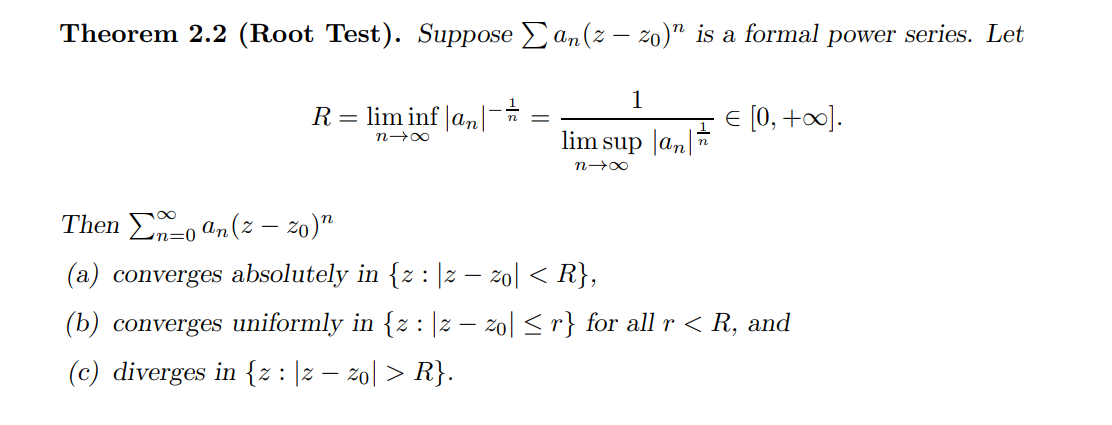
\includegraphics{figures/image_2021-05-27-15-40-58.png}
\caption{image\_2021-05-27-15-40-58}
\end{figure}

\end{proposition}

\begin{proposition}[Radius of Convergence by the Root Test]

For \(f(z) = \sum_{k\in {\mathbb{N}}} c_k z^k\), defining
\begin{align*}
{1\over R} \coloneqq\limsup_{k} {\left\lvert {a_k} \right\rvert}^{1\over k}
,\end{align*}
then \(f\) converges absolutely and uniformly for
\(D_R \coloneqq{\left\lvert {z} \right\rvert} < R\) and diverges for
\({\left\lvert {z} \right\rvert} > R\). Moreover \(f\) is holomorphic in
\(D_R\), can be differentiated term-by-term, and
\(f' = \sum_{k\in {\mathbb{N}}} n c_k z^k\).

\end{proposition}

\begin{fact}

Recall the \textbf{\(p{\hbox{-}}\)test}:
\begin{align*}
\sum n^{-p} < \infty \iff p \in (1, \infty)
.\end{align*}

\end{fact}

\begin{fact}

The product of two sequences is given by the Cauchy product
\begin{align*}
\sum a_kz^k \cdot \sum b_k z^k = \sum c_k z^k,\quad c_k \coloneqq\sum_{j\leq k} a_k b_{k-j}
.\end{align*}

\end{fact}

\begin{fact}

Recall how to carry out polynomial long division:

\todo[inline]{Polynomial long division}

\end{fact}

\begin{fact}[Partial Fraction Decomposition]

\envlist

\begin{itemize}
\tightlist
\item
  For every root \(r_i\) of multiplicity 1, include a term
  \(A/(x-r_i)\).
\item
  For any factors \(g(x)\) of multiplicity \(k\), include terms
  \(A_1/g(x), A_2/g(x)^2, \cdots, A_k / g(x)^k\).
\item
  For irreducible quadratic factors \(h_i(x)\), include terms of the
  form \({Ax+B \over h_i(x)}\).
\end{itemize}

\end{fact}

\hypertarget{exercises}{%
\subsection{Exercises}\label{exercises}}

\begin{exercise}[?]

Find the radius of convergences for the power series expansion of
\(\sqrt{z}\) about \(z_0 = 4 +3i\).

\end{exercise}

\hypertarget{preliminaries}{%
\section{Preliminaries}\label{preliminaries}}

\begin{definition}[Toy contour]

A closed Jordan curve that separates \({\mathbb{C}}\) into an exterior
and interior region is referred to as a \textbf{toy contour}.

\end{definition}

\begin{fact}[Complex roots of a number]

The complex \(n\)th roots of \(z \coloneqq r e^{i\theta}\) are given by
\begin{align*}
\left\{{ \omega_k \coloneqq r^{1/n} e^{i \qty{ \theta + 2k\pi \over n} } {~\mathrel{\Big|}~}0 \leq k \leq n-1 }\right\}
.\end{align*}
Note that one root is \(r^{1/n}\in {\mathbb{R}}\), and the rest are
separated by angles of \(2\pi/n\). Mnemonic:
\begin{align*}
z = re^{i\theta} = re^{i\qty{\theta + 2k\pi}} \implies z^{1/n} = \cdots
.\end{align*}

\end{fact}

\hypertarget{complex-log}{%
\subsection{Complex Log}\label{complex-log}}

\begin{fact}[Complex Log]

For \(z= r e^{i\theta}\neq 0\), \(\theta\) is of the form
\(\Theta + 2k\pi\) where \(\Theta = \operatorname{Arg}z\) We define
\begin{align*}
\log(z) = \ln\qty{{\left\lvert {z} \right\rvert}} + i\operatorname{Arg}(z)
\end{align*}
and \(z^c \coloneqq e^{c\log(z)}\). Thus
\begin{align*}
\log(re^{i\theta}) = \ln {\left\lvert {r} \right\rvert} + i\theta
.\end{align*}

\end{fact}

\begin{fact}

Common trick:
\begin{align*}
f^{1/n} = e^{{1\over n} \log(f)}
,\end{align*}
taking (say) a principal branch of \(\log\) given by
\({\mathbb{C}}\setminus(-\infty, 0] \times 0\).

\end{fact}

\begin{proposition}[Existence of complex log]

Suppose \(\Omega\) is a simply-connected region such that
\(1\in \Omega, 0\not\in\Omega\). Then there exists a branch of
\(F(z) \coloneqq\operatorname{Log}(z)\) such that

\begin{itemize}
\tightlist
\item
  \(F\) is holomorphic on \(\Omega\),
\item
  \(e^{F(z)} = z\) for all \(z\in \Omega\)
\item
  \(F(x) = \log(x)\) for \(x\in {\mathbb{R}}\) in a neighborhood of
  \(1\).
\end{itemize}

\end{proposition}

\begin{definition}[Principal branch and exponential]

Take \({\mathbb{C}}\) and delete \({\mathbb{R}}^{\leq 0}\) to obtain the
\textbf{principal branch} of the logarithm. Equivalently, this is define
for all \(z=re^{i\theta}\) where \(\theta \in (-\pi, \pi)\).

Here the log is defined as
\begin{align*}
\operatorname{Log}(z) \coloneqq\log(r) + i\theta && {\left\lvert {\theta} \right\rvert} < \pi
.\end{align*}
Similarly define
\begin{align*}
z^{\alpha} \coloneqq e^{\alpha \operatorname{Log}(z)}
.\end{align*}

\end{definition}

\begin{warnings}

It's tempting to define
\begin{align*}
z^{1\over n} \coloneqq(re^{i\theta})^{1\over n} = r^{1\over n} e^{i\theta \over n}
,\end{align*}
but this requires a branch cut to ensure continuity.

\end{warnings}

\begin{remark}

Note the problem: for \(z\coloneqq x+i0 \in {\mathbb{R}}^{\leq 0}\),
just above the axis consider \(z_+ \coloneqq x + i{\varepsilon}\) and
\(z_- \coloneqq x-i{\varepsilon}\). Then

\begin{itemize}
\tightlist
\item
  \(\log(z_+) = \log{\left\lvert {x} \right\rvert} + i\pi\), and
\item
  \(\log(z_-) = \log{\left\lvert {x} \right\rvert} - i\pi\).
\end{itemize}

So \(\log\) can't even be made continuous if one crosses the branch. The
issue is the \textbf{branch point} or \textbf{branch singularity} at
\(z=0\).

\end{remark}

\begin{theorem}[Existence of log of a function]

If \(f\) is holomorphic and nonvanishing on a simply-connected region
\(\Omega\), then there exists a holomorphic \(G\) on \(\Omega\) such
that
\begin{align*}
f(z) = e^{G(z)}
.\end{align*}

\end{theorem}

\hypertarget{complex-calculus}{%
\subsection{Complex Calculus}\label{complex-calculus}}

\begin{remark}

When parameterizing integrals \(\int_\gamma f(z)\,dz\), parameterize
\(\gamma\) by \(\theta\) and write \(z=re^{i\theta}\) so
\(\,dz= ire^{i\theta}\,d\theta\).

\end{remark}

\begin{warnings}

\(f(z) = \sin(z), \cos(z)\) are unbounded on \({\mathbb{C}}\)! An easy
way to see this: they are nonconstant and entire, thus unbounded by
Liouville.

\end{warnings}

\begin{example}[?]

You can show \(f(z) = \sqrt{z}\) is not holomorphic by showing its
integral over \(S^1\) is nonzero. This is a direct computation:
\begin{align*}
\int_{S^1} z^{1/2} \,dz
&= \int_0^{2\pi} (e^{i\theta})^{1/2} ie^{i\theta} \,d\theta\\
&= i \int_0^{2\pi} e^{i3\theta \over 2}\,d\theta\\
&= i \qty{2\over 3i} e^{i3\theta \over 2}\Big|_{0}^{2\pi} \\
&= {2\over 3}\qty{e^{3\pi i - 1}} \\
&= -{4\over 3}
.\end{align*}

Note an issue: a different parameterization yields a different (still
nonzero) number
\begin{align*}
\cdots 
&= \int_{-\pi}^{\pi} (e^{i\theta})^{1/2} ie^{i\theta} \,d\theta\\
&= {2\over 3}\qty{ e^{3\pi i \over 2} - e^{-3\pi i \over 2}} \\
&= -{4i\over 3}
.\end{align*}
This is these are paths that don't lift to closed loops on the Riemann
surface defined by \(z\mapsto z^2\).

\end{example}

\hypertarget{holomorphy-and-cauchy-riemann}{%
\subsubsection{Holomorphy and
Cauchy-Riemann}\label{holomorphy-and-cauchy-riemann}}

\begin{definition}[Analytic]

A function \(f:\Omega \to {\mathbb{C}}\) is \emph{analytic} at
\(z_0\in \Omega\) iff there exists a power series
\(g(z) = \sum a_n (z-z_0)^n\) with radius of convergence \(R>0\) and a
neighborhood \(U\ni z_0\) such that \(f(z) = g(z)\) on \(U\).

\end{definition}

\begin{definition}[Complex differentiable / holomorphic /entire]

A function \(f: {\mathbb{C}}\to {\mathbb{C}}\) is \textbf{complex
differentiable} or \textbf{holomorphic} at \(z_0\) iff the following
limit exists:
\begin{align*}
\lim_{h\to 0} { f(z_0 + h) - f(h) \over h  } 
.\end{align*}
A function that is holomorphic on \({\mathbb{C}}\) is said to be
\textbf{entire}.

Equivalently, there exists an \(\alpha\in {\mathbb{C}}\) such that
\begin{align*}
f(z_0+h) - f(z_0) = \alpha h + R(h) && R(h) \overset{h\to 0}\longrightarrow 0 
.\end{align*}
In this case, \(\alpha = f'(z_0)\).

\end{definition}

\begin{example}[Holomorphic vs non-holomorphic]

\envlist

\begin{itemize}
\tightlist
\item
  \(f(z) \coloneqq{\left\lvert {z} \right\rvert}\) is not holomorphic.
\item
  \(f(z) \coloneqq\arg{z}\) is not holomorphic.
\item
  \(f(z) \coloneqq\Re{z}\) is not holomorphic.
\item
  \(f(z) \coloneqq\Im{z}\) is not holomorphic.
\item
  \(f(z) = {1\over z}\) is holomorphic on
  \({\mathbb{C}}\setminus\left\{{0}\right\}\) but not holomorphic on
  \({\mathbb{C}}\)
\item
  \(f(z) = \mkern 1.5mu\overline{\mkern-1.5muz\mkern-1.5mu}\mkern 1.5mu\)
  is \emph{not} holomorphic, but is real differentiable:
  \begin{align*}
  {f(z_0 + h) - f(z_0) \over h } = {\mkern 1.5mu\overline{\mkern-1.5muz_0\mkern-1.5mu}\mkern 1.5mu + \mkern 1.5mu\overline{\mkern-1.5muh\mkern-1.5mu}\mkern 1.5mu - \mkern 1.5mu\overline{\mkern-1.5muz_0\mkern-1.5mu}\mkern 1.5mu \over h} = {\mkern 1.5mu\overline{\mkern-1.5muh\mkern-1.5mu}\mkern 1.5mu \over h} = {re^{-i\theta} \over re^{i\theta}} = e^{-2i\theta} \overset{h\to 0}\longrightarrow e^{-2i\theta}
  ,\end{align*}
  which is a complex number that depends on \(\theta\) and is thus not a
  single value.
\end{itemize}

\end{example}

\begin{definition}[Real (multivariate) differentiable]

A function \(F: {\mathbb{R}}^n\to {\mathbb{R}}^m\) is
\textbf{real-differentiable} at \(\mathbf{p}\) iff there exists a linear
transformation \(A\) such that
\begin{align*}
{ {\left\lVert { F(\mathbf{p} + \mathbf{h}) - F(\mathbf{p}) - A(\mathbf{h}) } \right\rVert} \over {\left\lVert { \mathbf{h} } \right\rVert} } \overset{{\left\lVert {\mathbf{h}} \right\rVert}\to 0}\longrightarrow 0
.\end{align*}
Rewriting,
\begin{align*}
{\left\lVert { F(\mathbf{p} + \mathbf{h}) - F(\mathbf{p})  - A(\mathbf{h}) } \right\rVert} = {\left\lVert { \mathbf{h} } \right\rVert} {\left\lVert { R(\mathbf{h}) } \right\rVert}
&& {\left\lVert {R(\mathbf{h}) } \right\rVert}\overset{{\left\lVert {\mathbf{h} } \right\rVert} \to 0}\longrightarrow 0
.\end{align*}

Equivalently,
\begin{align*}
F(\mathbf{p} + \mathbf{h}) - F(\mathbf{p}) = A(\mathbf{h}) + {\left\lVert {\mathbf{h}} \right\rVert} R(\mathbf{h}) && {\left\lVert {R(\mathbf{h}) } \right\rVert}\overset{{\left\lVert {\mathbf{h} } \right\rVert} \to 0}\longrightarrow 0
.\end{align*}

Or in a slightly more useful form,
\begin{align*}
F(\mathbf{p} + \mathbf{h}) = F(\mathbf{p}) + A(\mathbf{h}) + R(\mathbf{h}) && R\in o( {\left\lVert {\mathbf{h}} \right\rVert}), \text{ i.e. }
{ {\left\lVert { R(\mathbf{h}) } \right\rVert} \over  {\left\lVert {\mathbf{h}} \right\rVert}} \overset{\mathbf{h}\to 0}\longrightarrow 0
.\end{align*}

\end{definition}

\begin{proposition}[Complex differentiable implies Cauchy-Riemann]

If \(f\) is differentiable at \(z_0\), then the limit defining
\(f'(z_0)\) must exist when approaching from any direction. Identify
\(f(z) = f(x, y)\) and write \(z_0 = x+ iy\), then first consider
\(h\in RR\), so \(h = h_1 + ih_2\) with \(h_2 = 0\). Then
\begin{align*}
f'(z_0) = 
\lim_{h_1\to 0} { f(x+h_1, y) - f(x, y) \over h_1}
\coloneqq{\frac{\partial f}{\partial x}\,}(x, y)
.\end{align*}
Taking \(h \in i{\mathbb{R}}\) purely imaginary, so \(h= ih_2\),
\begin{align*}
f'(z_0)
= \lim_{ih_2\to 0} { f(x, y+h_2) - f(x, y) \over ih_2 } \coloneqq{1\over i} {\frac{\partial f}{\partial y}\,}(x, y)
.\end{align*}
Equating,
\begin{align*}
{\frac{\partial f}{\partial x}\,} = {1\over i} {\frac{\partial f}{\partial y}\,}
,\end{align*}
and writing \(f = u + iv\) and \(1/i = -i\) yields
\begin{align*}
{\frac{\partial f}{\partial x}\,} &= {\frac{\partial u}{\partial x}\,} + i {\frac{\partial v}{\partial x}\,} \\
{1\over i} {\frac{\partial f}{\partial y}\,} &= {1\over i} \qty{ {\frac{\partial u}{\partial y}\,} + i {\frac{\partial v}{\partial y}\,}} = {\frac{\partial v}{\partial y}\,} - i{\frac{\partial u}{\partial y}\,} 
.\end{align*}
Thus
\begin{align*}
{\frac{\partial u}{\partial x}\,} = {\frac{\partial v}{\partial y}\,} \hspace{8em} {\frac{\partial u}{\partial y}\,} = -{\frac{\partial v}{\partial x}\,}
.\end{align*}

\end{proposition}

\begin{proposition}[Polar Cauchy-Riemann equations]

\begin{align*}  
\frac{\partial u}{\partial r}=\frac{1}{r} \frac{\partial v}{\partial \theta} \quad \text { and } \quad \frac{1}{r} \frac{\partial u}{\partial \theta}=-\frac{\partial v}{\partial r}
.\end{align*}

\end{proposition}

\begin{proof}

Setting
\begin{align*}
z = re^{i\theta} = r(\cos(\theta) + i\sin(\theta) ) = x+iy
\end{align*}
yields \(x=r\cos(\theta), y=r\sin(\theta)\), one can identify
\begin{align*}
x_r = \cos(\theta)&, x_\theta = -r\sin(\theta) \\
y_r = \sin(\theta)&, y_\theta = r\cos(\theta)
.\end{align*}

Now apply the chain rule:
\begin{align*}
u_r 
&= u_x x_r + u_y y_r \\
&= v_y x_r -v_x y_r && \text{CR}\\
&= v_y \cos(\theta) - v_x \sin(\theta) \\
&= {1\over r}\qty{ v_y r\cos(\theta) - v_x r\sin(\theta) } \\
&= {1\over r}\qty { v_y y_\theta + v_x x_\theta} \\
&= {1\over r} v_\theta
.\end{align*}
Similarly,
\begin{align*}
v_r
&= v_x x_r + v_y y_r \\
&= v_x \cos(\theta) + v_y\sin(\theta) \\
&= -u_y\cos(\theta) + u_x\sin(\theta) && \text{CR} \\
&= {1\over r}\qty{ -u_y r\cos(\theta) + u_x r\sin(\theta)} \\
&= {1\over r}\qty{ -u_y y_\theta - u_x x_0 } \\
&= -{1\over r} u_\theta
.\end{align*}

Thus
\begin{align*}
\frac{\partial u}{\partial r}=\frac{1}{r} \frac{\partial v}{\partial \theta} \quad \text { and } \quad \frac{\partial v}{\partial r}=-\frac{1}{r} \frac{\partial u}{\partial \theta} \\
.\end{align*}

\end{proof}

\begin{proposition}[Holomorphic functions are continuous.]

\(f\) is holomorphic at \(z_0\) iff there exists an
\(a\in {\mathbb{C}}\) such that
\begin{align*}  
f(z_0 + h) - f(z_0) - ah = h \psi(h), \quad \psi(h) \overset{h\to 0}\to 0
.\end{align*}
In this case, \(a = f'(z_0)\).

\end{proposition}

\todo[inline]{Prove}

\hypertarget{delbar-and-the-laplacian}{%
\subsubsection{Delbar and the
Laplacian}\label{delbar-and-the-laplacian}}

\begin{definition}[del and delbar operators]

\begin{align*}
{\partial}\coloneqq{\partial}_z \coloneqq{1\over 2}\qty{{\partial}_x - i {\partial}_y}
\quad
\text{ and }
\quad
{ \mkern 1.5mu\overline{\mkern-1.5mu{\partial}\mkern-1.5mu}\mkern 1.5mu}
\coloneqq{\partial}_{\mkern 1.5mu\overline{\mkern-1.5muz\mkern-1.5mu}\mkern 1.5mu}
={1\over 2}\qty{ {\partial}_x + i{\partial}_y}
.\end{align*}
Moreover,
\(f' = {\partial}f + { \mkern 1.5mu\overline{\mkern-1.5mu{\partial}\mkern-1.5mu}\mkern 1.5mu}f\).

\end{definition}

\begin{proposition}[Holomorphic iff delbar vanishes]

\(f\) is holomorphic at \(z_0\) iff
\({ \mkern 1.5mu\overline{\mkern-1.5mu{\partial}\mkern-1.5mu}\mkern 1.5mu}f(z_0) = 0\):
\begin{align*}
2{ \mkern 1.5mu\overline{\mkern-1.5mu{\partial}\mkern-1.5mu}\mkern 1.5mu}f 
&\coloneqq({\partial}_x + i {\partial}_y) (u+iv) \\
&= u_x + iv_x + iu_y - v_y \\
&= (u_x - v_y) + i(u_y + v_x) \\
&= 0 && \text{by Cauchy-Riemann}
.\end{align*}

\end{proposition}

\hypertarget{harmonic-functions-and-the-laplacian}{%
\subsubsection{Harmonic Functions and the
Laplacian}\label{harmonic-functions-and-the-laplacian}}

\begin{definition}[Laplacian and Harmonic Functions]

A real function of two variables \(u(x, y)\) is \textbf{harmonic} iff it
is in the kernel of the Laplacian operator:
\begin{align*}  
\Delta u \coloneqq\qty{{\frac{\partial ^2}{\partial x^2}\,} + {\frac{\partial ^2}{\partial y^2}\,}}u = 0
.\end{align*}

\end{definition}

\begin{proposition}[Cauchy-Riemann implies holomorphic]

If \(f = u+iv\) with \(u, v\in C^1({\mathbb{R}})\) satisfying the
Cauchy-Riemann equations on \(\Omega\), then \(f\) is holomorphic on
\(\Omega\) and
\begin{align*}
f'(z) = {\partial}f = {1\over 2}\qty{u_x + iv_x}
.\end{align*}

\end{proposition}

\begin{proposition}[Holomorphic functions have harmonic components]

If \(f(z) = u(x, y) + iv(x, y)\) is holomorphic, then \(u, v\) are
harmonic.

\end{proposition}

\begin{proof}[?]

\envlist

\begin{itemize}
\item
  By CR,
  \begin{align*}
  u_x = v_y && u_y = -v_x
  .\end{align*}
\item
  Differentiate with respect to \(x\):
  \begin{align*}
  u_{xx} = v_{yx} && u_{yx} = -v_{xx}
  .\end{align*}
\item
  Differentiate with respect to \(y\):
  \begin{align*}
  u_{xy} = v_{yy} && u_{yy} = -v_{xy}
  .\end{align*}
\item
  Clairaut's theorem: partials are equal, so
  \begin{align*}
  u_{xx} - v_{yx} = 0 \implies u_{xx} + u_{yy} = 0 \\ \\
  v_{xx} + u_{yx} = 0 \implies v_{xx} + v_{yy} = 0 \\ \\
  .\end{align*}
\end{itemize}

\end{proof}

\hypertarget{exercises-1}{%
\subsubsection{Exercises}\label{exercises-1}}

\begin{proposition}[Injectivity Relates to Derivatives]

If \(z_0\) is a zero of \(f'\) of order \(n\), then \(f\) is
\((n+1)\)-to-one in a neighborhood of \(z_0\).

\end{proposition}

\begin{proof}

?

\end{proof}

\todo[inline]{proof}

\begin{exercise}[Zero derivative implies constant]

Show that if \(f' = 0\) on a domain \(\Omega\), then \(f\) is constant
on \(\Omega\)

\end{exercise}

\begin{solution}

Write \(f = u + iv\), then \(0 = 2 f' = u_x + iv_x = u_y - iu_y\), so
\(\operatorname{grad}u = \operatorname{grad}v = 0\). Show \(f\) is
constant along every straight line segment \(L\) by computing the
directional derivative \(\operatorname{grad}u \cdot \mathbf{v} = 0\)
along \(L\) connecting \(p, q\). Then \(u(p) = u(q) = a\) some constant,
and \(v(p) = v(q) = b\), so \(f(z) = a+bi\) everywhere.

\end{solution}

\begin{exercise}[f and fbar holomorphic implies constant]

Show that if \(f\) and
\(\mkern 1.5mu\overline{\mkern-1.5muf\mkern-1.5mu}\mkern 1.5mu\) are
both holomorphic on a domain \(\Omega\), then \(f\) is constant on
\(\Omega\).

\end{exercise}

\begin{solution}

\envlist

\begin{itemize}
\item
  Strategy: show \(f'=0\).
\item
  Write \(f = u + iv\). Since \(f\) is analytic, it satisfies CR, so
  \begin{align*}
  u_x = v_y && u_y = -v_x
  .\end{align*}
\item
  Similarly write
  \(\mkern 1.5mu\overline{\mkern-1.5muf\mkern-1.5mu}\mkern 1.5mu = U + iV\)
  where \(U = u\) and \(V = -v\). Since
  \(\mkern 1.5mu\overline{\mkern-1.5muf\mkern-1.5mu}\mkern 1.5mu\) is
  analytic, it also satisfies CR , so
  \begin{align*}
  U_x = V_y && U_y = -V_x \\ \\
  \implies u_x = -v_y && u_y = v_x
  .\end{align*}
\item
  Add the LHS of these two equations to get
  \(2u_x = 0 \implies u_x = 0\). Subtract the right-hand side to get
  \(-2v_x = 0 \implies v_x = 0\)
\item
  Since \(f\) is analytic, it is holomorphic, so \(f'\) exists and
  satisfies \(f' = u_x + iv_x\). But by above, this is zero.
\item
  By the previous exercise, \(f'=0 \implies f\) is constant.
\end{itemize}

\end{solution}

\begin{exercise}[SS 1.13: Constant real/imaginary/magnitude implies constant]

If \(f\) is holomorphic on \(\Omega\) and any of the following hold,
then \(f\) is constant:

\begin{enumerate}
\def\labelenumi{\arabic{enumi}.}
\tightlist
\item
  \(\Re(f)\) is constant.
\item
  \(\Im(f)\) is constant.
\item
  \({\left\lvert {f} \right\rvert}\) is constant.
\end{enumerate}

\end{exercise}

\begin{solution}

\textbf{Part 3}:

\begin{itemize}
\tightlist
\item
  Write \({\left\lvert {f} \right\rvert} = c \in {\mathbb{R}}\).
\item
  If \(c=0\), done, so suppose \(c>0\).
\item
  Use
  \(f\mkern 1.5mu\overline{\mkern-1.5muf\mkern-1.5mu}\mkern 1.5mu = {\left\lvert {f} \right\rvert}^2 = c^2\)
  to write
  \(\mkern 1.5mu\overline{\mkern-1.5muf\mkern-1.5mu}\mkern 1.5mu=c^2/f\).
\item
  Since \({\left\lvert {f(z)} \right\rvert} = 0 \iff f(z) = 0\), we have
  \(f\neq 0\) on \(\Omega\), so
  \(\mkern 1.5mu\overline{\mkern-1.5muf\mkern-1.5mu}\mkern 1.5mu\) is
  analytic.
\item
  Similarly \(f\) is analytic, and
  \(f,\mkern 1.5mu\overline{\mkern-1.5muf\mkern-1.5mu}\mkern 1.5mu\)
  analytic implies \(f'=0\) implies \(f\) is constant.
\end{itemize}

\end{solution}

\todo[inline]{Finish}

\hypertarget{power-series}{%
\subsection{Power Series}\label{power-series}}

\begin{theorem}[Improved Taylor's Theorem]

If \(f\) is holomorphic on a region \(\Omega\) with
\(\overline{ D_R(z_0)} \subseteq \Omega\), and for every
\(z\in D_r(z_0)\), \(f\) has a power series expansion of the following
form:
\begin{align*}
f(z)=\sum_{n=0}^{\infty} a_{n}\left(z-z_{0}\right)^{n} \quad\text{ where } a_{n}=\frac{f^{(n)}\left(z_{0}\right)}{n !}
= {1 \over 2\pi r^n}\int_0^{2\pi} f(z_0 + re^{i\theta})e^{-in\theta} \,d\theta
.\end{align*}

\end{theorem}

\begin{proposition}[Power Series are Smooth]

Any power series is smooth (and thus holomorphic) on its disc of
convergence, and its derivatives can be obtained using term-by-term
differentiation:
\begin{align*}
{\frac{\partial }{\partial z}\,} f(z) = {\frac{\partial }{\partial z}\,} \sum_{k\geq 0} c_k (z-z_0)^k = \sum_{k\geq 1} kc_k (z-z_0)^k
.\end{align*}
Moreover, the coefficients are given by
\begin{align*}
c_k = {f^{(n)}(z_0) \over n! }
.\end{align*}

\end{proposition}

\begin{remark}

By an application of the Cauchy integral formula (see S\&S 7.1) if \(f\)
is holomorphic on \(D_R(z_0)\) there is a formula for all \(k\geq 0\)
and all \(0<r<R\):
\begin{align*}
c_k = {1\over 2\pi r^k} \int_0^{2\pi} f(z_0 + re^{i\theta}) e^{-in\theta}\,d\theta
.\end{align*}

\end{remark}

\begin{proposition}[Exponential is uniformly convergent in discs]

\(f(z) = e^z\) is uniformly convergent in any disc in \({\mathbb{C}}\).

\end{proposition}

\begin{proof}

Apply the estimate
\begin{align*}  
{\left\lvert {e^z} \right\rvert} \leq \sum {{\left\lvert {z} \right\rvert}^n \over n!} = e^{{\left\lvert {z} \right\rvert}}
.\end{align*}
Now by the \(M{\hbox{-}}\)test,
\begin{align*}  
{\left\lvert {z} \right\rvert} \leq R < \infty \implies {\left\lvert {\sum {z^n \over n!}} \right\rvert} \leq e^R < \infty
.\end{align*}

\end{proof}

\begin{lemma}[Dirichlet's Test]

Given two sequences of real numbers
\(\left\{{ a_k }\right\} , \left\{{ b_k }\right\}\) which satisfy

\begin{enumerate}
\def\labelenumi{\arabic{enumi}.}
\tightlist
\item
  The sequence of partial sums \(\left\{{ A_n }\right\}\) is bounded,
\item
  \(b_k \searrow 0\).
\end{enumerate}

then
\begin{align*}
\sum_{k\geq 1} a_k b_k < \infty
.\end{align*}

\end{lemma}

\begin{proof}[?]

\begin{quote}
See \url{http://www.math.uwaterloo.ca/~krdavids/Comp/Abel.pdf}
\end{quote}

Use summation by parts. For a fixed \(\sum a_k b_k\), write
\begin{align*}
\sum_{n=1}^m x_n Y_n + \sum_{n=1}^m X_n y_{n+1} = X_m Y_{m+1}
.\end{align*}
Set \(x_n \coloneqq a_n, y_N \coloneqq b_n - b_{n-1}\), so \(X_n = A_n\)
and \(Y_n = b_n\) as a telescoping sum. Importantly, all \(y_n\) are
negative, so
\({\left\lvert {y_n} \right\rvert} = {\left\lvert {b_n - b_{n-1}} \right\rvert} = b_{n-1} - b_n\),
and moreover \(a_n b_n = x_n Y_n\) for all \(n\). We have
\begin{align*}
\sum_{n\geq 1} a_n b_n 
&= \lim_{N\to\infty} \sum_{n\leq N} x_n Y_n \\
&= \lim_{N\to\infty} \sum_{n\leq N} X_N Y_N - \sum_{n\leq N} X_n y_{n+1} \\
&= - \sum_{n\geq 1} X_n y_{n+1},
\end{align*}
where in the last step we've used that
\begin{align*}
{\left\lvert {X_N} \right\rvert} = {\left\lvert {A_N} \right\rvert}\leq M \implies {\left\lvert {X_N Y_{N} } \right\rvert} = {\left\lvert {X_N} \right\rvert} {\left\lvert {b_{n+1}} \right\rvert} \leq M b_{n+1} \to 0
.\end{align*}
So it suffices to bound the latter sum:
\begin{align*}
\sum_{k\geq n}{\left\lvert { X_k y_{k+1} } \right\rvert} 
&\leq M \sum_{k\geq 1} {\left\lvert {y_{k+1}} \right\rvert}\\
&\leq M \sum_{k\geq 1} b_{k} - b_{k+1} \\
&\leq 2M(b_1 - b_{n+1})\\
&\leq 2M b_1
.\end{align*}

\end{proof}

\begin{theorem}[Abel's Theorem]

If \(\sum_{k=1}^\infty c_k z^j\) converges on
\({\left\lvert {z} \right\rvert} < 1\) then
\begin{align*}
\lim_{z\to 1^-} \sum_{k\in {\mathbb{N}}} c_k z^k = \sum_{k\in {\mathbb{N}}} c_k
.\end{align*}

\end{theorem}

\begin{lemma}[Abel's Test]

If \(f(z) \coloneqq\sum c_k z^k\) is a power series with
\(c_k \in {\mathbb{R}}^{\geq 0}\) and \(c_k\searrow 0\), then \(f\)
converges on \(S^1\) except possibly at \(z=1\).

\end{lemma}

\begin{example}[application of Abel's theorem]

What is the value of the alternating harmonic series? Integrate a
geometric series to obtain
\begin{align*}
\sum {(-1)^k z^k \over n} = \log(z+1) && {\left\lvert {z} \right\rvert} < 1
.\end{align*}
Since \(c_k \coloneqq(-1)^k/k \searrow 0\), this converges at \(z=1\),
and by Abel's theorem \(f(1) = \log(2)\).

\end{example}

\begin{remark}

The converse to Abel's theorem is false: take
\(f(z) = \sum (-z)^n = 1/(1+z)\). Then \(f(1) = 1-1+1-\cdots\) diverges
at 1, but \(1/1+1 = 1/2\). So the limit
\(s\coloneqq\lim_{x\to 1^-} f(x) 1/2\), but \(\sum a_n\) doesn't
converge to \(s\).

\end{remark}

\begin{proposition}[Summation by Parts]

Setting \(A_n \coloneqq\sum_{k=1}^n b_k\) and \(B_0 \coloneqq 0\),
\begin{align*}
\sum_{k=m}^n a_k b_k 
&= A_nb_n - A_{m-1} b_m - \sum_{k=m}^{n-1} A_k(b_{k+1} - b_{k})
.\end{align*}
Compare this to integrating by parts:
\begin{align*}
\int_a^b f g = F(b)g(b) - F(a)g(a) - \int_a^b Fg'
.\end{align*}

Note there is a useful form for taking the product of sums:
\begin{align*}
A_{n} B_{n}=\sum_{k=1}^{n} A_{k} b_{k}+\sum_{k=1}^{n} a_{k} B_{k-1}
.\end{align*}

\end{proposition}

\begin{proof}[?]

An inelegant proof: define \(A_n \coloneqq\sum_{k\leq n} a_k\), use that
\(a_k = A_k - A_{k-1}\), reindex, and peel a top/bottom term off of each
sum to pattern-match.\\

Behold:
\begin{align*}
\sum_{m\leq k \leq n} a_k b_k 
&= \sum_{m\leq k \leq n} (A_k - A_{k-1}) b_k \\
&= \sum_{m\leq k \leq n} A_kb_k - \sum_{m\leq k \leq n} A_{k-1} b_k \\
&= \sum_{m\leq k \leq n} A_kb_k - \sum_{m-1\leq k \leq n-1} A_{k} b_{k+1} \\
&= A_nb_n + \sum_{m\leq k \leq n-1} A_kb_k - \sum_{m-1\leq k \leq n-1} A_{k} b_{k+1} \\
&= A_nb_n - A_{m-1} b_{m} + \sum_{m\leq k \leq n-1} A_kb_k - \sum_{m\leq k \leq n-1} A_{k} b_{k+1} \\
&= A_nb_n - A_{m-1} b_{m} + \sum_{m\leq k \leq n-1} A_k(b_k - b_{k+1}) \\
&= A_nb_n - A_{m-1} b_{m} - \sum_{m\leq k \leq n-1} A_k(b_{k+1} - b_{k}) 
.\end{align*}

\end{proof}

\begin{proposition}[?]

If \(f\) is non-constant, then \(f'\) is analytic and the zeros of
\(f'\) are isolated. If \(f,g\) are analytic with \(f'=g'\), then
\(f-g\) is constant.

\end{proposition}

\hypertarget{exercises-series}{%
\subsubsection{Exercises: Series}\label{exercises-series}}

\begin{exercise}[Application of summation by parts]

Use summation by parts to show that \(\sin(n)/n\) converges.

\end{exercise}

\begin{exercise}[1.20: Series convergence on the circle]

Show that

\begin{enumerate}
\def\labelenumi{\arabic{enumi}.}
\tightlist
\item
  \(\sum kz^k\) diverges on \(S^1\).
\item
  \(\sum k^{-2} z^k\) converges on \(S^1\).
\item
  \(\sum k^{-1}z^k\) converges on \(S^1\setminus\left\{{1}\right\}\) and
  diverges at \(1\).
\end{enumerate}

\end{exercise}

\begin{solution}

\begin{enumerate}
\def\labelenumi{\arabic{enumi}.}
\tightlist
\item
  Use that \({\left\lvert {z^k} \right\rvert} = 1\) and
  \(\sum c_kz^k < \infty \implies {\left\lvert {c_k} \right\rvert} \to 0\),
  but
  \({\left\lvert {kz^k} \right\rvert} = {\left\lvert {k} \right\rvert} \to \infty\)
  here.
\item
  Use that absolutely convergent implies convergent, and
  \(\sum {\left\lvert {k^{-2} z^k} \right\rvert} = \sum {\left\lvert {k^{-2}} \right\rvert}\)
  converges by the \(p{\hbox{-}}\)test.
\item
  If \(z=1\), this is the harmonic series. Otherwise take
  \(a_k = 1/k, b_k = e^{i k \theta}\) where \(\theta \in (0, 2\pi)\) is
  some constant, and apply Dirichlet's test. It suffices to bound the
  partial sums of the \(b_k\). Recalling that
  \(\sum_{k\leq N} r^k = (1-r^{N+1}) / (1-r)\),
  \begin{align*}
    {\left\lVert { \sum_{k\leq m} e^{ik\theta } } \right\rVert} = {\left\lVert {1 - e^{i(m+1)\theta} \over 1 - e^{i\theta}} \right\rVert} \leq {2 \over {\left\lVert { 1- e^{i\theta}} \right\rVert}} \coloneqq M
    ,\end{align*}
  which is a constant. Here we've used that two points on \(S^1\) are at
  most distance 2 from each other.
\end{enumerate}

\end{solution}

\begin{exercise}[Laurent expansions inside and outside of a disc]

Expand \(f(z) = {1\over z(z-1)}\) in both

\begin{itemize}
\tightlist
\item
  \({\left\lvert {z} \right\rvert} < 1\)
\item
  \({\left\lvert {z} \right\rvert} > 1\)
\end{itemize}

\end{exercise}

\begin{solution}

\begin{align*}
{1\over z(z-1)} = -{1\over z}{1 \over 1-z} = -{1\over z}\sum z^k
.\end{align*}
and
\begin{align*}
{1\over z(z-1)} = {1\over z^2(1 - {1\over z})} = {1\over z^2} \sum \qty{1\over z}^k
.\end{align*}

\end{solution}

\begin{exercise}[Laurent expansions about different points]

Find the Laurent expansion about \(z=0\) and \(z=1\) respectively of the
following function:
\begin{align*}
f(z) \coloneqq{z+1 \over z(z-1)}
.\end{align*}

\end{exercise}

\begin{solution}

Note: once you see that everything is in terms of powers of \((z-z_0)\),
you're essentially done. For \(z=0\):
\begin{align*}
{z+1 \over z(z-1)}
&= {1\over z} {z+1 \over z-1} \\
&= -{z+1\over z} {1\over 1-z} \\
&= -\qty{1 + {1\over z}}\sum_{k\geq 0} z^k
.\end{align*}

For \(z=1\):
\begin{align*}
{z+1 \over z(z-1)}
&= {1\over z-1}\qty{1 + {1\over z} } \\
&= {1\over z-1}\qty{1 + {1\over 1 - (1-z)} } \\
&= {1\over z-1} \qty{1 + \sum_{k\geq 0} (1-z)^k } \\
&= {1\over z-1} \qty{1 + \sum_{k\geq 0} (-1)^k (z-1)^k }
.\end{align*}

\end{solution}

\begin{exercise}[?]

Show that a real-valued holomorphic function must be constant.

\end{exercise}

\hypertarget{cauchys-theorem}{%
\section{Cauchy's Theorem}\label{cauchys-theorem}}

\hypertarget{complex-integrals}{%
\subsection{Complex Integrals}\label{complex-integrals}}

\begin{definition}[Complex Integral]

\begin{align*}
\int_{\gamma} f d z:=\int_{I} f(\gamma(t)) \gamma^{\prime}(t) \,dt
= \int_\gamma (u+iv)\,dx\wedge (-v+iu)\,dy
.\end{align*}

\end{definition}

\begin{theorem}[Cauchy-Goursat Theorem]\label{CauchyTheorem}

If \(f\) is holomorphic on a region \(\Omega\) with
\(\pi_1 \Omega = 1\), then for any closed path
\(\gamma \subseteq \Omega\),
\begin{align*} 
\int_{\gamma} f(z) \,dz= 0
.\end{align*}

\end{theorem}

\begin{slogan}

Closed path integrals of holomorphic functions vanish.

\end{slogan}

\hypertarget{applications-of-cauchys-theorem}{%
\subsection{Applications of Cauchy's
Theorem}\label{applications-of-cauchys-theorem}}

\hypertarget{integral-formulas-and-estimates}{%
\subsubsection{Integral Formulas and
Estimates}\label{integral-formulas-and-estimates}}

\begin{quote}
See
\href{http://home.iitk.ac.in/~psraj/mth102/lecture_notes/comp8.pdf}{reference}
\end{quote}

\begin{theorem}[Cauchy Integral Formula]\label{CauchyIntegral}

Suppose \(f\) is holomorphic on \(\Omega\), then for any
\(z_0 \in \Omega\) and any open disc \(\overline{D_R(z_0)}\) such that
\(\gamma \coloneqq{{\partial}}\overline{D_R(z_0)} \subseteq \Omega\),
\begin{align*}
f(z_0) = {1 \over 2\pi i} \int_{\gamma} {f(\xi) \over \xi-z_0}\ \,d\xi
\end{align*}
and
\begin{align*}
{\frac{\partial ^nf }{\partial z^n}\,}(z_0) = {n! \over 2\pi i} \int_{\gamma} {f(\xi) \over (\xi - z_0)^{n+1}} \,d\xi
.\end{align*}

\end{theorem}

\begin{proof}[?]

\begin{figure}
\centering
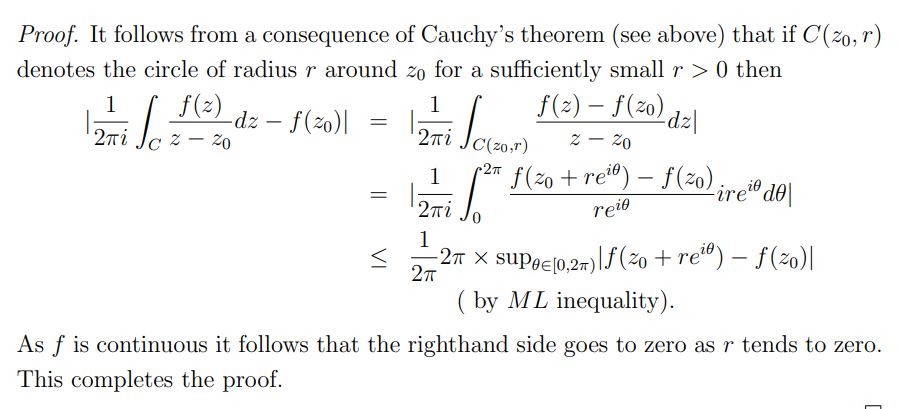
\includegraphics{figures/image_2021-05-27-16-54-06.png}
\caption{image\_2021-05-27-16-54-06}
\end{figure}

\end{proof}

\begin{proof}[?]

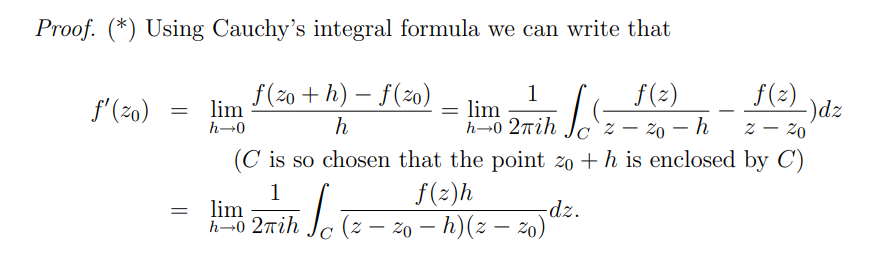
\includegraphics{figures/image_2021-05-27-16-56-39.png}
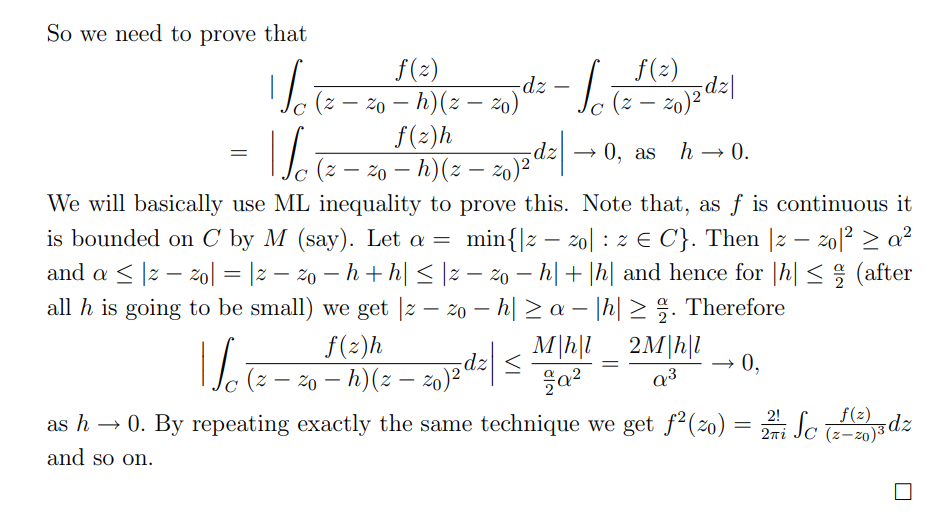
\includegraphics{figures/image_2021-05-27-16-56-52.png}

\end{proof}

\begin{theorem}[Cauchy's Inequality / Cauchy's Estimate]\label{CauchyInequality}

For \(z_0 \in D_R(z_0) \subset \Omega\), setting
\(M \coloneqq\sup_{z\in \gamma}{\left\lvert {f(z)} \right\rvert}\) so
\({\left\lvert {f(z)} \right\rvert}\leq M\) on \(\gamma\)
\begin{align*}
{\left\lvert { f^{(n)} (z_0) } \right\rvert} 
\leq \frac{n !}{2 \pi} \int_{0}^{2 \pi} \frac{ M } {R^{n+1}} R \,d\theta
= \frac{M n ! }{R^n} 
.\end{align*}

\end{theorem}

\begin{proof}[of Cauchy's inequality]

\envlist

\begin{itemize}
\tightlist
\item
  Given \(z_0\in \Omega\), pick the largest disc
  \(D_R(z_0) \subset \Omega\) and let \(C = {{\partial}}D_R\).
\item
  Then apply the integral formula.
\end{itemize}

\begin{align*}
\left|f^{(n)}(z_0)\right|
&= {\left\lvert { \frac{n !}{2 \pi i} \int_{C} \frac{f(\zeta) }{(\zeta-z_0)^{n+1}} \,d\zeta} \right\rvert} \\
&=\left|\frac{n !}{2 \pi i} \int_{0}^{2 \pi} \frac{f\left(z_0 + r e^{i \theta}\right) r i e^{i \theta} }{\left(r e^{i \theta}\right)^{n+1}} \,d\theta\right| \\
&\leq \frac{n !}{2 \pi} \int_{0}^{2 \pi}\left|\frac{f\left( z_0 +r e^{i \theta}\right) r i e^{i \theta}}{\left(r e^{i \theta}\right)^{n+1}}\right| \,d\theta\\ 
&=\frac{n !}{2 \pi} \int_{0}^{2 \pi} \frac{\left|f\left(z_0 +r e^{i \theta}\right)\right|}{r^{n}} \,d\theta\\
&\leq \frac{n !}{2 \pi} \int_{0}^{2 \pi} \frac{M}{r^{n}} \,d\theta\\
&=\frac{M n !}{r^{n}} 
.\end{align*}

\end{proof}

\begin{slogan}

The \(n\)th Taylor coefficient of an analytic function is at most
\(\sup_{{\left\lvert {z} \right\rvert} = R} {\left\lvert {f} \right\rvert}/R^n\).

\end{slogan}

\begin{theorem}[Mean Value Property for Holomorphic Functions]

If \(f\) is holomorphic on \(D_r(z_0)\)
\begin{align*}
f(z_0) 
= {1\over 2\pi} \int_0^{2\pi} f(z_0 + re^{i\theta}) \,d\theta
= {1\over \pi r^2} \iint_{D_r(z_0)} f(z)\, dA
.\end{align*}
Taking the real part of both sides, one can replace \(f=u+iv\) with
\(u\).

\end{theorem}

\hypertarget{liouville}{%
\subsubsection{Liouville}\label{liouville}}

\begin{theorem}[Liouville's Theorem]\label{Liouville}

If \(f\) is entire and bounded, \(f\) is constant.

\end{theorem}

\begin{proof}[of Liouville]

\envlist

\begin{itemize}
\tightlist
\item
  Since \(f\) is bounded, \(f(z) \leq M\) uniformly on \({\mathbb{C}}\).
\item
  Apply Cauchy's estimate for the 1st derivative:
  \begin{align*}
  {\left\lvert {f'(z)} \right\rvert} \leq { 1! {\left\lVert {f} \right\rVert}_{C_R} \over R } \leq {M \over R}\overset{R\to\infty}\longrightarrow 0
  ,\end{align*}
  so \(f'(z) = 0\) for all \(z\).
\end{itemize}

\end{proof}

\begin{exercise}[?]

\begin{figure}
\centering
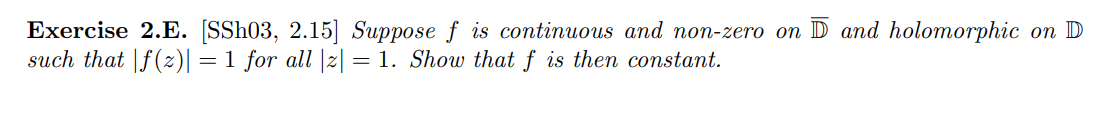
\includegraphics{figures/image_2021-05-17-11-54-14.png}
\caption{image\_2021-05-17-11-54-14}
\end{figure}

\end{exercise}

\hypertarget{continuation-principle}{%
\subsubsection{Continuation Principle}\label{continuation-principle}}

\begin{theorem}[Continuation Principle / Identity Theorem]

If \(f\) is holomorphic on a bounded connected domain \(\Omega\) and
there exists a sequence \(\left\{{z_i}\right\}\) with a limit point in
\(\Omega\) such that \(f(z_i) = 0\), then \(f\equiv 0\) on \(\Omega\).

\end{theorem}

\begin{slogan}

Two functions agreeing on a set with a limit point are equal on a
domain.

\end{slogan}

\begin{proof}[?]

Apply Improved Taylor Theorem? \todo[inline]{todo}

\end{proof}

\begin{exercise}[?]

\begin{figure}
\centering
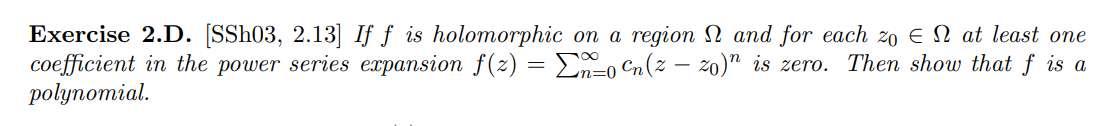
\includegraphics{figures/image_2021-05-17-11-53-33.png}
\caption{image\_2021-05-17-11-53-33}
\end{figure}

\end{exercise}

\hypertarget{exercises-2}{%
\subsection{Exercises}\label{exercises-2}}

\begin{exercise}[Primitives imply vanishing integral]

Show that if \(f\) has a primitive \(F\) on \(\Omega\) then
\(\int_\gamma f = 0\) for every closed curve
\(\gamma \subseteq \Omega\).

\end{exercise}

\begin{exercise}[?]

Prove the uniform limit theorem for holomorphic functions: if
\(f_n\to f\) locally uniformly and each \(f_n\) is holomorphic then
\(f\) is holomorphic.

\end{exercise}

\begin{solution}

This is S\&S Theorem 5.2. Statement: if \(f_n\to f\) uniformly locally
uniformly on \(\Omega\) then \(f\) is holomorphic on \(\Omega\).

\envlist

\begin{itemize}
\tightlist
\item
  Let \(D \subset \Omega\) with
  \(\mkern 1.5mu\overline{\mkern-1.5mu{\mathbb{D}}\mkern-1.5mu}\mkern 1.5mu\subset \Omega\)
  and \(\Delta \subset D\) be a triangle.
\item
  Apply Goursat: \(\int_\Delta f_n = 0\).
\item
  \(f_n\to f\) uniformly on \(\Delta\) since it is closed and bounded
  and thus compact by Heine-Borel, so \(f\) is continuous and
  \begin{align*}
  \lim_n \int_\Delta f_n = \int_\Delta \lim_n f_n \coloneqq\int_\Delta f
  .\end{align*}
\item
  Apply Morera's theorem: \(\int_\Delta f\) vanishes on every triangle
  in \(\Omega\), so \(f\) is holomorphic on \(\Omega\).
\end{itemize}

\end{solution}

\begin{exercise}[?]

Prove that if \(f_n\to f\) locally uniformly with \(f_n\) holomorphic,
then \(f_n'\to f'\) locally uniformly and \(f'\) is holomorphic.

\end{exercise}

\begin{solution}

\envlist

\begin{itemize}
\item
  Simplifying step: for some reason, it suffices to assume \(f_n\to f\)
  uniformly on all of \(\Omega\)?
\item
  Take \(\Omega_R\) to be \(\Omega\) with a buffer of \(R\), so
  \(d(z, {{\partial}}\Omega) > R\) for every
  \(z \in \mkern 1.5mu\overline{\mkern-1.5mu\Omega_R\mkern-1.5mu}\mkern 1.5mu\).
\item
  It suffices to show the following bound for \(F\) any holomorphic
  function on \(\Omega\):
  \begin{align*}
  \sup_{z\in \Omega_R} {\left\lvert {F'(z)} \right\rvert} \leq {1\over R} \sup_{\zeta \in \Omega} {\left\lvert {F(\zeta)} \right\rvert} && \forall R
  ,\end{align*}
  where on the right we take the sup over all \(\Omega\).

  \begin{itemize}
  \tightlist
  \item
    Then take \(F \coloneqq f_n-f\) and \(R\to 0\) to conclude, since
    the right-hand side is a constant not depending on \(\Omega_R\).
  \end{itemize}
\item
  For any \(z\in \Omega_R\), we have
  \(\mkern 1.5mu\overline{\mkern-1.5muD_R(z)\mkern-1.5mu}\mkern 1.5mu \subseteq \Omega_R\),
  so Cauchy's integral formula can be applied:
\item

  \begin{align*}
  {\left\lvert {F'(z)} \right\rvert} 
  &= {\left\lvert { {1\over 2\pi i} \int_{{{\partial}}D_R(z)} {F(\xi) \over (\xi-z)^2 } \,d\xi} \right\rvert} \\
  &\leq {1\over 2\pi} \int_{{{\partial}}D_R(z)} { { {\left\lvert {F(\xi)} \right\rvert} \over {\left\lvert {\xi-z} \right\rvert}^2 }} \,d\xi\\
  &\leq {1\over 2\pi} \int_{{{\partial}}D_R(z)} { { \sup_{\zeta\in \Omega} {\left\lvert {F(\zeta)} \right\rvert} \over {\left\lvert {\xi-z} \right\rvert}^2 }} \,d\xi\\
  &= {1\over 2\pi} \sup_{\zeta\in \Omega} {\left\lvert {F(\zeta)} \right\rvert}  \int_{{{\partial}}D_R(z)} { { 1 \over R^2 }} \,d\xi\\
  &= {1\over 2\pi} \sup_{\zeta\in \Omega} {\left\lvert {F(\zeta)} \right\rvert}  {1\over R^2} \int_{{{\partial}}D_R(z)} \,d\xi\\
  &= {1\over 2\pi} \sup_{\zeta\in \Omega} {\left\lvert {F(\zeta)} \right\rvert}  {1\over R^2} 2\pi R   \\
  &\leq {1\over 2\pi} \sup_{\zeta\in \Omega} {\left\lvert {F(\zeta)} \right\rvert}  {1\over R^2}\qty{ 2\pi R}   \\
  &= {1\over R} \sup_{\zeta \in \Omega}{\left\lvert {F(\zeta)} \right\rvert}
  .\end{align*}
\item
  Now
  \begin{align*}
  {\left\lVert {f_n' - f'} \right\rVert}_{\infty, \Omega_R} \leq {1\over R} {\left\lVert {f_n - f} \right\rVert}_{\infty, \Omega}
  ,\end{align*}
  where if \(R\) is fixed then by uniform convergence of \(f_n\to f\),
  for \(n\) large enough
  \({\left\lVert {f_n - f} \right\rVert} < {\varepsilon}/R\).
\end{itemize}

\end{solution}

\hypertarget{moreras-theorem}{%
\subsection{Morera's Theorem}\label{moreras-theorem}}

\begin{theorem}[Morera's Theorem]\label{Morera}

If \(f\) is continuous on a domain \(\Omega\) and \(\int_T f = 0\) for
every triangle \(T\subset \Omega\), then \(f\) is holomorphic.

\end{theorem}

\begin{slogan}

If every integral along a triangle vanishes, implies holomorphic.

\end{slogan}

\begin{corollary}[Sufficient condition for a sequence to converge to a holomorphic function]

If \(\left\{{ f_n }\right\}_{n\in {\mathbb{N}}}\) is a holomorphic
sequence on a region \(\Omega\) which uniformly converges to \(f\) on
every compact subset \(K \subseteq \Omega\), then \(f\) is holomorphic,
and \(f_n' \to f'\) uniformly on every such compact subset \(K\).

\end{corollary}

\begin{proof}[?]

Commute limit with integral and apply Morera's theorem.

\end{proof}

\begin{remark}

This can be applied to series of the form \(\sum_k f_k(z)\).

\end{remark}

\hypertarget{symmetric-regions}{%
\subsubsection{Symmetric Regions}\label{symmetric-regions}}

In this section, take \(\Omega\) to be a region symmetric about the real
axis, so
\(z\in \Omega \iff \mkern 1.5mu\overline{\mkern-1.5muz\mkern-1.5mu}\mkern 1.5mu \in \Omega\).
Partition this set as
\(\Omega^+ \subseteq {\mathbb{H}}, I \subseteq {\mathbb{R}}, \Omega^- \subseteq \mkern 1.5mu\overline{\mkern-1.5mu{\mathbb{H}}\mkern-1.5mu}\mkern 1.5mu\).

\begin{theorem}[Symmetry Principle]

Suppose that \(f^+\) is holomorphic on \(\Omega^+\) and \(f^-\) is
holomorphic on \(\Omega^-\), and \(f\) extends continuously to \(I\)
with \(f^+(x) = f^-(x)\) for \(x\in I\). Then the following
piecewise-defined function is holomorphic on \(\Omega\):
\begin{align*}
f(z) 
\coloneqq
\begin{cases}
f^+(z) & z\in \Omega^+ 
\\
f^-(z) & z\in \Omega^-
\\
f^+(z) = f^-(z) & z\in I.
\end{cases}
\end{align*}

\end{theorem}

\begin{proof}[?]

Apply Morera?

\end{proof}

\begin{theorem}[Schwarz Reflection ]\label{SchwarzReflection}

If \(f\) is continuous and holomorphic on \({\mathbb{H}}^+\) and
real-valued on \({\mathbb{R}}\), then the extension defined by
\(F^-(z) = \mkern 1.5mu\overline{\mkern-1.5muf(\mkern 1.5mu\overline{\mkern-1.5muz\mkern-1.5mu}\mkern 1.5mu)\mkern-1.5mu}\mkern 1.5mu\)
for \(z\in {\mathbb{H}}^-\) is a well-defined holomorphic function on
\({\mathbb{C}}\).

\end{theorem}

\begin{proof}[?]

Apply the symmetry principle.

\end{proof}

\begin{remark}

\({\mathbb{H}}^+, {\mathbb{H}}^-\) can be replaced with any region
symmetric about a line segment \(L\subseteq {\mathbb{R}}\).

\end{remark}

\hypertarget{zeros-and-singularities}{%
\section{Zeros and Singularities}\label{zeros-and-singularities}}

\begin{definition}[Singularity]

A point \(z_0\) is an \textbf{isolated singularity} if \(f(z_0)\) is
undefined but \(f(z)\) is defined in a punctured neighborhood
\(D(z_0)\setminus\left\{{z_0}\right\}\) of \(z_0\).

There are three types of isolated singularities:

\begin{itemize}
\tightlist
\item
  Removable singularities
\item
  Poles
\item
  Essential singularities
\end{itemize}

\end{definition}

\begin{definition}[Removable Singularities]

If \(z_0\) is a singularity of \(f\). then \(z_0\) is a
\textbf{removable singularity} iff there exists a holomorphic function
\(g\) such that \(f(z) = g(z)\) in a punctured neighborhood of \(z_0\).
Equivalently,
\begin{align*}
\lim_{z\to z_0}(z-z_0) f(z) = 0
.\end{align*}
Equivalently, \(f\) is bounded on a neighborhood of \(z_0\).

\end{definition}

\begin{remark}

Singularities can be classified by Laurent expansions
\(f(z) = \sum_{k\in {\mathbb{Z}}} c_k z^k\):

\begin{itemize}
\tightlist
\item
  Essential singularity: infinitely many negative terms.
\item
  Pole of order \(N\): truncated at \(k = -N\), so \(c_{N-\ell} = 0\)
  for all \(\ell\).
\item
  Removable singularity: truncated at \(k=0\), so \(c_{\leq -1} = 0\).
\end{itemize}

\end{remark}

\begin{example}[Removable singularities]

\envlist

\begin{itemize}
\tightlist
\item
  \(f(z) \coloneqq\sin(z)/z\) has a removable singularity at \(z=0\),
  and one can redefine \(f(0) \coloneqq 1\).
\item
  If \(f(z) = p(z)/q(z)\) with \(q(z_0)=0\) and \(p(z_0)=0\), then
  \(z_0\) is removable with \(f(z_0)\coloneqq p'(z_0)/q'(z_0)\).
\end{itemize}

\end{example}

\begin{example}[Essential singularities]

\(f(z) \coloneqq e^{1/z}\) has an essential singularity at \(z=0\),
since we can expand and pick up infinitely many negative terms:
\begin{align*}
e^{1/z} = 1 + {1\over z} + {1\over 2! z^2} + \cdots
.\end{align*}
In fact there exists a neighborhood of zero such that
\(f(U) = {\mathbb{C}}\setminus\left\{{0}\right\}\). Similarly
\(g(z) \coloneqq\sin\qty{1\over z}\) has an essential singularity at
\(z=0\), and there is a neighborhood \(V\) of zero such that
\(g(V) = {\mathbb{C}}\).

\end{example}

\begin{example}[?]

The singularities of a rational function are always isolated, since
there are finitely many zeros of any polynomial. The function
\(F(z) \coloneqq\operatorname{Log}(z)\) has a singularity at \(z=0\)
that is \textbf{not} isolated, since every neighborhood intersects the
branch cut \((-\infty, 0) \times\left\{{ 0 }\right\}\), where \(F\) is
not even defined. The function \(G(z) \coloneqq 1/\sin(\pi/z)\) has a
non-isolated singularity at 0 and isolated singularities at \(1/n\) for
all \(n\).

\end{example}

\begin{warnings}

\(f(z) \coloneqq z^{1\over 2}\) has a singularity at zero that does not
fall under this classification -- \(z=0\) is a \textbf{branch
singularity} and admits no Laurent expansion around \(z=0\).

A similar example: \(\qty{z(z-1)}^{1\over 2}\) has two branch
singularities at \(z=0, 1\).

\end{warnings}

\begin{theorem}[Extension over removable singularities]

If \(f\) is holomorphic on \(\Omega\setminus\left\{{z_0}\right\}\) where
\(z_0\) is a removable singularity, then there is a unique holomorphic
extension of \(f\) to all of \(\Omega\).

\end{theorem}

\begin{proof}[?]

Take \(\gamma\) to be a circle centered at \(z_0\) and use
\begin{align*}
f(z) \coloneqq\int_\gamma { f(\xi) \over \xi - z} \,dx
.\end{align*}
This is valid for \(z\neq z_0\), but the right-hand side is analytic.
(?)

\end{proof}

\todo[inline]{Revisit}

\begin{theorem}[Improved Taylor Remainder Theorem]

If \(f\) is analytic on a region \(\Omega\) containing \(z_0\), then
\(f\) can be written as
\begin{align*}
f(z)
=\left(\sum_{k=0}^{n-1} \frac{f^{(k)}\left(z_{0}\right)}{k !}\left(z-z_{0}\right)^{k}\right)+ 
R_{n}(z)\left(z-z_{0}\right)^{n}
,\end{align*}
where \(R_n\) is analytic.

\end{theorem}

\begin{definition}[Zeros]

If \(f\) is analytic and not identically zero on \(\Omega\) with
\(f(z_0) = 0\), then there exists a nonvanishing holomorphic function
\(g\) such that
\begin{align*}
f(z) = (z-z_0)^n g(z)
.\end{align*}
We refer to \(z_0\) as a \textbf{zero of order \(n\)}.

\end{definition}

\begin{definition}[Poles (and associated terminology)]

A \emph{pole} \(z_0\) of a function \(f(z)\) is a zero of
\(g(z) \coloneqq{1\over f(z)}\). Equivalently,
\(\lim_{z\to z_0} f(z) = \infty\). In this case there exists a minimal
\(n\) and a holomorphic \(h\) such that
\begin{align*}  
f(z) = \qty{z-z_0}^{-n} h(z)
.\end{align*}
Such an \(n\) is the \emph{order} of the pole. A pole of order 1 is said
to be a \emph{simple pole}.

\end{definition}

\begin{definition}[Principal Part and Residue]

If \(f\) has a pole of order \(n\) at \(z_0\), then there exist a
holomorphic \(G\) in a neighborhood of \(z_0\) such that
\begin{align*}
f(z) = {a_{-n} \over (z-z_0)^n } + \cdots + {a_{-1} \over z-z_0} + G(z) \coloneqq P(z) + G(z)
.\end{align*}

The term \(P(z)\) is referred to as the \emph{principal part of \(f\) at
\(z_0\)} consists of terms with negative degree, and the \emph{residue}
of \(f\) at \(z_0\) is the coefficient \(a_{-1}\).

\end{definition}

\begin{definition}[Essential Singularity]

A singularity \(z_0\) is \emph{essential} iff it is neither removable
nor a pole. Equivalently, a Laurent series expansion about \(z_0\) has a
principal part with infinitely many terms.

\end{definition}

\begin{theorem}[Casorati-Weierstrass]\label{Casorati}

If \(f\) is holomorphic on \(\Omega\setminus\left\{{z_0}\right\}\) where
\(z_0\) is an essential singularity, then for every
\(V\subset \Omega\setminus\left\{{z_0}\right\}\), \(f(V)\) is dense in
\({\mathbb{C}}\).

\end{theorem}

\begin{slogan}

The image of a punctured disc at an essential singularity is dense in
\({\mathbb{C}}\).

\end{slogan}

\begin{proof}[of Casorati-Weierstrass]

Pick \(w\in {\mathbb{C}}\) and suppose toward a contradiction that
\(D_R(w) \cap f(V)\) is empty. Consider
\begin{align*}
g(z) \coloneqq{1\over f(z) - w}
,\end{align*}
and use that it's bounded to conclude that \(z_0\) is either removable
or a pole for \(f\).

\end{proof}

\begin{definition}[Singularities at infinity]

For any \(f\) holomorphic on an unbounded region, we say \(z=\infty\) is
a singularity (of any of the above types) of \(f\) if
\(g(z) \coloneqq f(1/z)\) has a corresponding singularity at \(z=0\).

\end{definition}

\begin{definition}[Meromorphic]

A function \(f:\Omega\to{\mathbb{C}}\) is \emph{meromorphic} iff there
exists a sequence \(\left\{{z_n}\right\}\) such that

\begin{itemize}
\tightlist
\item
  \(\left\{{z_n}\right\}\) has no limit points in \(\Omega\).
\item
  \(f\) is holomorphic in \(\Omega\setminus\left\{{z_n}\right\}\).
\item
  \(f\) has poles at the points \(\left\{{z_n}\right\}\).
\end{itemize}

Equivalently, \(f\) is holomorphic on \(\Omega\) with a discrete set of
points delete which are all poles of \(f\).

\end{definition}

\begin{theorem}[Meromorphic implies rational]

Meromorphic functions on \({\mathbb{C}}\) are rational functions.

\end{theorem}

\begin{proof}[?]

Consider \(f(z) - P(z)\), subtracting off the principal part at each
pole \(z_0\), to get a bounded entire function and apply Liouville.

\end{proof}

\begin{theorem}[Riemann Extension Theorem]

A singularity of a holomorphic function is removable if and only if the
function is bounded in some punctured neighborhood of the singular
point.

\end{theorem}

\hypertarget{counting-zeros-and-poles}{%
\section{Counting Zeros and Poles}\label{counting-zeros-and-poles}}

\hypertarget{argument-principle}{%
\subsection{Argument Principle}\label{argument-principle}}

\begin{definition}[The logarithmic derivative]

The \textbf{logarithmic derivative} is defined as
\begin{align*}
{\partial}_{\log} f \coloneqq{f' \over f}
.\end{align*}
It converts all poles and zeros of \(f\) into simple poles of
\({\partial}_{\log f}\).

\end{definition}

\begin{exercise}[?]

Show that
\({\partial}_{\log}(fg) = {\partial}_{\log} f + {\partial}_{\log} g\),
i.e.~
\begin{align*}
{ (fg)' \over fg} = {f'\over f} + {g' \over g}
.\end{align*}

\end{exercise}

\begin{definition}[Winding Number]

For \(\gamma \subseteq \Omega\) a closed curve not passing through a
point \(z_0\), the \textbf{winding number of \(\gamma\) about \(z_0\)}
(or the \textbf{index}) is defined as
\begin{align*}
\mathop{\mathrm{Ind}}_{z=z_0}(\gamma) \coloneqq{1\over 2\pi i} \int_\gamma {1\over \xi -z_0}\,d\xi
.\end{align*}

\end{definition}

\begin{theorem}[Argument Principle, Zeros/Poles Version]

For \(f\) meromorphic in \(\Omega\) with multisets of zeros
\(Z_f \coloneqq\left\{{ z_j }\right\}\) and poles
\(P_f\coloneqq\left\{{ p_k }\right\}\) (so repeated with multiplicity)
for \(\gamma \coloneqq{{\partial}}\Omega\) not intersect
\begin{align*}  
{1\over 2\pi i} \int_\gamma {\partial}_{\log} f(z) \,dz
&= \# Z_f - \# P_f
,\end{align*}
where \(\# Z_f\) and \(\# P_f\) are the number of zeros and poles
respectively, counted with multiplicity.

\end{theorem}

\begin{proof}[?]

\envlist

\begin{itemize}
\item
  If \(z_0\) is a zero of \(f\) of order \(m\), write
  \(f(z) = (z-z_0)^m g(z)\) with \(g(z)\) holomorphic and nonzero on
  some neighborhood of \(z_0\).
\item
  Compute
  \begin{align*}
  {\partial}_{\log} f(z)
  &=
  \frac{m\left(z-z_{0}\right)^{m-1} g(z)+\left(z-z_{0}\right)^{m} g^{\prime}(z)}{\left(z-z_{0}\right)^{m} g(z)} \\
  &= {m \over z-z_0} + {\partial}_{\log} g(z)
  ,\end{align*}
  so \(z_0\) is a simple pole of \({\partial}_{\log} f\) and
  \(\mathop{\mathrm{res}}_{z=z_0} {\partial}_{\log} f = m\).
\item
  If \(z_0\) is a pole of \(f\) of order \(m\), write
  \(f(z) = (z-z_0)^{-m} g(z)\), then
  \begin{align*}
  {\partial}_{\log} f = {-m \over z-z_0} + {\partial}_{\log} g
  ,\end{align*}
  so \(z_0\) is a simple pole and
  \(\mathop{\mathrm{Res}}_{z=z_0} {\partial}_{\log f} = -m\).
\item
  Now apply the residue theorem, and group residues according to sign:
  \begin{align*}
  {1\over 2\pi i } \int_{\gamma} {\partial}_{\log }f(z) \,dz
  &= \sum_{z_i \in P_{{\partial}_{\log} f}} \mathop{\mathrm{Res}}_{z=z_i} {\partial}_{\log} f(z)\\
  &= \sum_{z_k \in Z_f} \mathop{\mathrm{Res}}_{z=z_k} f(z) - \sum_{z_j \in P_f} \mathop{\mathrm{Res}}_{z=z_j} f(z)
  .\end{align*}
\end{itemize}

\end{proof}

\begin{theorem}[Argument Principle, Index Version]

With the same setup as above,
\begin{align*}
{1\over 2\pi i} \int_\gamma {\partial}_{\log} f(z) \,dz
&= \mathop{\mathrm{Ind}}_{w=0}(f\circ \gamma)(w)
.\end{align*}

\end{theorem}

\begin{proof}[?]

Make the change of variables \(w = f(z)\), then
\(z=\gamma(t) \mapsto w = (f\circ \gamma)(t)\) and \(\,dw= f'(z) \,dz\),
so
\begin{align*}
{1\over 2\pi i }\int_{\gamma} {\partial}_{\log} f(z) \,dz
= {1\over 2\pi i} \int_{f\circ \gamma} {1\over w} \,dw\coloneqq\mathop{\mathrm{Ind}}_{w=0} (f\circ \gamma)(w)
.\end{align*}

\end{proof}

\begin{example}[Using the index version of the argument principle]

Let \(f(z) = z^2 + z = z(z+1)\).

\begin{itemize}
\tightlist
\item
  \(\gamma_1 \coloneqq\left\{{{\left\lvert {z} \right\rvert} = 2}\right\}\)
  contains 2 zeros and 0 poles, so \(f\circ \gamma\) winds twice around
  zero counterclockwise.
\item
  \(\gamma_2 \coloneqq\left\{{{\left\lvert {z} \right\rvert} = {1\over 2}}\right\}\)
  contains 1 zero and 0 poles, so \(f\circ \gamma\) winds once.
\end{itemize}

\end{example}

\hypertarget{rouchuxe9}{%
\subsection{Rouché}\label{rouchuxe9}}

\begin{theorem}[Rouché's Theorem]\label{Rouche}

If

\begin{itemize}
\tightlist
\item
  \(f, g\) are meromorphic on \(\Omega\)
\item
  \(\gamma \subset \Omega\) is a toy contour winding about each
  zero/pole of \(f, g\) exactly once,
\item
  \({\left\lvert {g} \right\rvert} < {\left\lvert {f} \right\rvert}\) on
  \(\gamma\)
\end{itemize}

then
\begin{align*}
\mathop{\mathrm{Ind}}_{z=0}(f\circ \gamma)(z) = \mathop{\mathrm{Ind}}_{z=0}((f+g)\circ \gamma)(z) \implies Z_f - P_f = Z_{f+g} - P_{f+g}
.\end{align*}
In particular, if \(f, g\) are holomorphic, they have the same number of
zeros in \(\Omega\).

\end{theorem}

\begin{slogan}

The number of zeros/poles are determined by a dominating function.

\end{slogan}

\todo[inline]{Prove}

\begin{exercise}[?]

Show that \(h(z) =z^5 + 3z + 1\) has 5 zeros in
\({\left\lvert {z} \right\rvert} \leq 2\).

\end{exercise}

\begin{exercise}[?]

Show that \(h(z) = z + 3 + 2e^z\) has one root in
\(\left\{{ \Re(z) \leq 0}\right\}\).

\end{exercise}

\begin{solution}

Use the following contour:

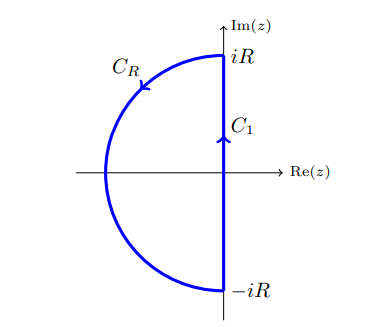
\includegraphics{figures/2021-07-29_20-39-31.png}

Take \(g(z) \coloneqq 2e^z < f(z) \coloneqq f(z) \coloneqq z+3\).

\end{solution}

\begin{corollary}[Open Mapping]

Any holomorphic non-constant map is an open map.

\end{corollary}

\todo[inline]{Prove}

\begin{corollary}[Maximum Modulus]\label{MaximumModulus}

If \(f\) is holomorphic and nonconstant on an open connected region
\(\Omega\), then \({\left\lvert {f} \right\rvert}\) can not attain a
maximum on \(\Omega\). If \(\Omega\) is bounded and \(f\) is continuous
on
\(\mkern 1.5mu\overline{\mkern-1.5mu\Omega\mkern-1.5mu}\mkern 1.5mu\),
then
\(\max_{\mkern 1.5mu\overline{\mkern-1.5mu\Omega\mkern-1.5mu}\mkern 1.5mu} {\left\lvert {f} \right\rvert}\)
occurs on \({{\partial}}\Omega\). Conversely, if \(f\) attains a local
supremum at \(z_0 \in \Omega\), then \(f\) is constant on \(\Omega\).

\end{corollary}

\todo[inline]{Prove}

\begin{corollary}[?]

If \(f\) is nonzero on \(\Omega\), then \(f\) attains a minimum on
\({{\partial}}\Omega\). This follows from applying the MMP to \(1/f\).

\end{corollary}

\hypertarget{counting-zeros}{%
\subsection{Counting Zeros}\label{counting-zeros}}

\begin{example}

\envlist

\begin{itemize}
\tightlist
\item
  Take \(P(z) = z^4 + 6z + 3\).
\item
  On \({\left\lvert {z} \right\rvert} < 2\):

  \begin{itemize}
  \tightlist
  \item
    Set \(f(z) = z^4\) and \(g(z) = 6z + 3\), then
    \({\left\lvert {g(z)} \right\rvert} \leq 6{\left\lvert {z} \right\rvert} + 3 = 15 < 16= {\left\lvert {f(z)} \right\rvert}\).
  \item
    So \(P\) has 4 zeros here.
  \end{itemize}
\item
  On \({\left\lvert {z} \right\rvert} < 1\):

  \begin{itemize}
  \tightlist
  \item
    Set \(f(z) = 6z\) and \(g(z) = z^4 + 3\).
  \item
    Check
    \({\left\lvert {g(z)} \right\rvert} \leq {\left\lvert {z} \right\rvert}^4 + 3 = 4 < 6 = {\left\lvert {f(z)} \right\rvert}\).
  \item
    So \(P\) has 1 zero here.
  \end{itemize}
\end{itemize}

\end{example}

\begin{example}

\envlist

\begin{itemize}
\tightlist
\item
  Claim: the equation \(\alpha z e^z = 1\) where
  \({\left\lvert {\alpha} \right\rvert} > e\) has exactly one solution
  in \({\mathbb{D}}\).
\item
  Set \(f(z) = \alpha z\) and \(g(z) = e^{-z}\).
\item
  Estimate at \({\left\lvert {z} \right\rvert} =1\) we have
  \({\left\lvert {g} \right\rvert} ={\left\lvert {e^{-z}} \right\rvert} = e^{-\Re(z)} \leq e^1 < {\left\lvert {\alpha} \right\rvert} = {\left\lvert {f(z)} \right\rvert}\)
\item
  \(f\) has one zero at \(z_0 = 0\), thus so does \(f+g\).
\end{itemize}

\end{example}

\hypertarget{residues}{%
\section{Residues}\label{residues}}

\hypertarget{basics}{%
\subsection{Basics}\label{basics}}

\begin{remark}

Check: do you need residues at all?? You may be able to just compute an
integral!

\begin{itemize}
\item
  Directly by parameterization:
  \begin{align*}
  \int_\gamma f \,dz= \int_a^b f(z(t))\, z'(t) \,dt&& \text{for } z(t) \text{ a parameterization of } \gamma
  ,\end{align*}
\item
  Finding a primitive \(F\), then
  \begin{align*}
  \int_\gamma f = F(b) - F(a)
  .\end{align*}

  \begin{itemize}
  \tightlist
  \item
    Note: you can parameterize a circle around \(z_0\) using
    \begin{align*}
    z= z_0 + re^{i \theta }
    .\end{align*}
  \end{itemize}
\end{itemize}

\end{remark}

\begin{fact}[Integrating $z^k$ around $S^1$ powers residues]

The major fact that reduces integrals to residues:
\begin{align*}
\int_\gamma z^k \,dz= \int_0^{2\pi} e^{ik\theta} ie^{i\theta } \,d\theta= i\int_0^{2\pi} e^{i(k+1)\theta \,d\theta}
=
\begin{cases}
2\pi i & k=-1 
\\
0 & \text{else}.
\end{cases}
\end{align*}
Thus
\begin{align*}
\int \sum_{k\geq -M} c_k z^k = \sum_{k\geq -M} \int c_k z^k = 2\pi i c_{-1}
,\end{align*}
i.e.~the integral picks out the \(c_{-1}\) coefficient in a Laurent
series expansion.

\end{fact}

\begin{example}[?]

Consider
\begin{align*}
f(z) \coloneqq{e^{iz} \over 1 + z^2}
\end{align*}
where \(z\neq \pm i\), and attempt to integrate
\begin{align*}
\int_{\mathbb{R}}f(z) \,dz
.\end{align*}
Use a semicircular contour \(\gamma_R\) where \(z = Re^{it}\) and check
\begin{align*}
\sup_{z\in \gamma_R} {\left\lvert {f(z)} \right\rvert} 
&= \max_{t\in [0, \pi} {1 \over 1 + (Re^{it})^2 } \\
&= \max_{t\in [0, \pi} {1 \over 1 + R^2e^{2it} } \\
&= {1\over R^2 - 1}
.\end{align*}

\end{example}

\hypertarget{estimates}{%
\subsection{Estimates}\label{estimates}}

\begin{proposition}[Length bound / ML Estimate]

\begin{align*}
{\left\lvert { \int_\gamma f} \right\rvert} \leq ML \coloneqq\sup_{z\in \gamma} {\left\lvert {f} \right\rvert} \cdot \mathrm{length}(\gamma)
.\end{align*}

\end{proposition}

\begin{proof}[?]

\begin{align*}
\left|\int_{\gamma} f(z) d z\right| \leq \sup _{t \in[a, b]}|f(z(t))| \int_{a}^{b}\left|z^{\prime}(t)\right| d t \leq \sup _{z \in \gamma}|f(z)| \cdot \operatorname{length}(\gamma)
.\end{align*}

\end{proof}

\begin{proposition}[Jordan's Lemma]

Suppose that \(f(z) = e^{iaz}g(z)\) for some \(g\), and let
\(C_R \coloneqq\left\{{ z=Re^{it} {~\mathrel{\Big|}~}t\in [0, \pi] }\right\}\).
Then
\begin{align*}
{\left\lvert {\int_{C_R} f(z) \,dz} \right\rvert} \leq {\pi M_R \over a}
\end{align*}
where
\(M_R \coloneqq\sup_{t\in [0, \pi]} {\left\lvert {g(Re^{it})} \right\rvert}\).

\end{proposition}

\begin{proof}[?]

\begin{align*}
{\left\lvert { \int_{C_R} f(z)\,dz} \right\rvert}
&= {\left\lvert { \int_{C_R} e^{iaz}g(z) \,dz} \right\rvert} \\
&= {\left\lvert { \int_{[0, \pi]} e^{ia\qty{Re^{it}}}g(Re^{it}) iRe^{it} \,dt} \right\rvert} \\
&\leq \int_{[0, \pi]} {\left\lvert { e^{ia\qty{Re^{it}}}g(Re^{it}) iRe^{it}} \right\rvert} \,dt\\
&=R \int_{[0, \pi]} {\left\lvert { e^{ia\qty{Re^{it}}}g(Re^{it})} \right\rvert} \,dt\\
&\leq R M_R \int_{[0, \pi]} {\left\lvert { e^{ia\qty{Re^{it}}}} \right\rvert} \,dt\\
&= R M_R \int_{[0, \pi]} e^{\Re\qty{iaRe^{it}}}   \,dt\\
&= R M_R \int_{[0, \pi]} e^{\Re\qty{iaR\qty{\cos(t) + i\sin(t) } }}   \,dt\\
&= R M_R \int_{[0, \pi]} e^{-aR\sin(t) }   \,dt\\
&= 2 R M_R \int_{[0, \pi/2]} e^{-aR\sin(t) }   \,dt\\
&\leq 2R M_R \int_{[0, \pi/2]} e^{-aR\qty{2t\over \pi} }   \,dt\\
&= 2RM_R \qty{\pi \over 2aR}\qty{1-e^{-aR}} \\
&= {\pi M_R \over a}
.\end{align*}

where we've used that on \([0, \pi/2]\), there is an inequality
\(2t/\pi \leq \sin(t)\). This is obvious from a picture, since
\(\sin(t)\) is a height on \(S^1\) and \(2t/\pi\) is a height on a
diagonal line:

\begin{figure}
\centering
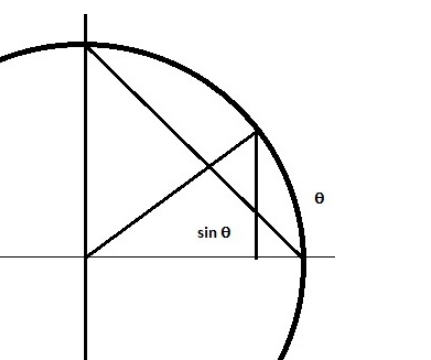
\includegraphics{figures/image_2021-06-09-01-29-22.png}
\caption{image\_2021-06-09-01-29-22}
\end{figure}

\end{proof}

\hypertarget{residue-formulas}{%
\subsection{Residue Formulas}\label{residue-formulas}}

\begin{theorem}[The Residue Theorem]

Let \(f\) be meromorphic on a region \(\Omega\) with poles
\(\left\{{ { {z}_1, {z}_2, \cdots, {z}_{N}} }\right\}\). Then for any
\(\gamma \in \Omega\setminus\left\{{ { {z}_1, {z}_2, \cdots, {z}_{N}} }\right\}\),
\begin{align*}
{1 \over 2\pi i } \int_\gamma f(z) \,dz= \sum_{j=1}^N n_\gamma(z_j) \mathop{\mathrm{Res}}_{z=z_j} f
.\end{align*}
If \(\gamma\) is a toy contour, then\\
\begin{align*}
{1\over 2\pi i}\int_\gamma f\,dz= \sum_{j=1}^N \mathop{\mathrm{Res}}_{z=z_j}f
.\end{align*}

\end{theorem}

\begin{proposition}[Residue formula for higher order poles]

If \(f\) has a pole \(z_0\) of order \(n\), then
\begin{align*}  
\mathop{\mathrm{Res}}_{z=z_0} f = \lim_{z\to z_0} {1 \over (n-1)!} \qty{{\frac{\partial }{\partial z}\,}}^{n-1} (z-z_0)^n f(z)
.\end{align*}

\end{proposition}

\begin{proposition}[Residue formula for simple poles]

As a special case, if \(z_0\) is a simple pole of \(f\), then
\begin{align*}  
\mathop{\mathrm{Res}}_{z=z_0}f = \lim_{z\to z_0} (z-z_0) f(z)
.\end{align*}

\end{proposition}

\begin{corollary}[Better derivative formula that sometimes works for simple poles]

If additionally \(f=g/h\) where \(h(z_0) = 0\) and \(h'(z_0)\neq 0\),
\begin{align*}
\mathop{\mathrm{Res}}_{z=z_0} {g(z) \over h(z)} = {g(z_0) \over h'(z_0)}
.\end{align*}

\end{corollary}

\begin{proof}[?]

Apply L'Hopital:
\begin{align*}
(z-z_0) {g(z) \over h(z)} = {(z-z_0) g(z) \over h(z) } \overset{LH}{=}
{g(z) + (z-z_0) g'(z) \over h'(z)} \overset{z\to z_0}\longrightarrow{g(z_0) \over h'(z_0)}
.\end{align*}

\end{proof}

\begin{example}[Residue of a simple pole (order 1)]

Let \(f(z) = \frac{1}{1+z^2}\), then \(g(z) = 1, h(z) = 1+z^2\), and
\(h'(z) = 2z\) so that \(h'(i) = 2i \neq 0\). Thus
\begin{align*}
\mathop{\mathrm{Res}}_{z=i}{1\over 1+z^2} = \frac{1}{2i}
.\end{align*}

\end{example}

\begin{proposition}[Residue at infinity]

\begin{align*}
\mathop{\mathrm{Res}}_{z=\infty}f(z) = \mathop{\mathrm{Res}}_{z=0} g(z) && g(z) \coloneqq-{1 \over z^2}f\qty{1\over z} 
.\end{align*}

\end{proposition}

\hypertarget{exercises-3}{%
\subsubsection{Exercises}\label{exercises-3}}

\begin{quote}
Some good computations
\href{https://math.mit.edu/~jorloff/18.04/notes/topic9.pdf}{here}.
\end{quote}

\begin{exercise}

Show that the complex zeros of \(f(z) \coloneqq\sin(\pi z)\) are exactly
\({\mathbb{Z}}\), and each is order 1. Calculate the residue of
\(1/\sin(\pi x)\) at \(z=n\in {\mathbb{Z}}\).

\end{exercise}

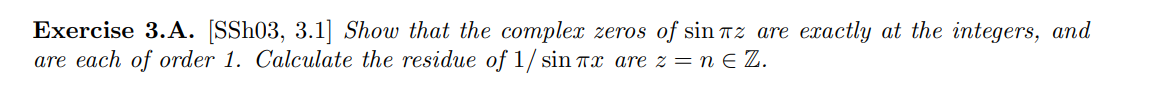
\includegraphics{figures/image_2021-05-17-13-32-46.png}
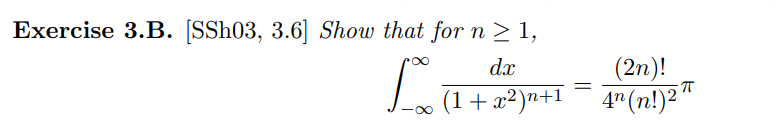
\includegraphics{figures/image_2021-05-17-13-32-57.png}
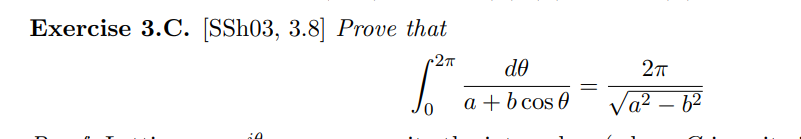
\includegraphics{figures/image_2021-05-17-13-33-12.png}
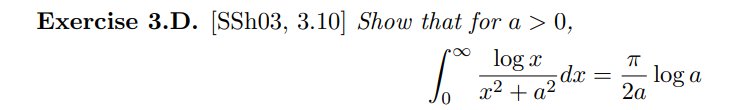
\includegraphics{figures/image_2021-05-17-13-33-30.png}

\begin{exercise}[?]

\begin{align*}
\int_{\mathbb{R}}{1 \over (1+x^2)^2} \,dx
.\end{align*}

\end{exercise}

\begin{solution}

\envlist

\begin{itemize}
\tightlist
\item
  Factor \((1+z^2)^2 = ((z-i)(z+i))^2\), so \(f\) has poles at \(\pm i\)
  of order 2.
\item
  Take a semicircular contour \(\gamma \coloneqq I_R \cup D_R\), then
  \(f(z) \approx 1/z^4 \to 0\) for large \(R\) and
  \(\int_{D_R} f \to 0\).
\item
  Note \(\int_{I_R} f \to \int_{\mathbb{R}}f\), so
  \(\int_\gamma f \to \int_{\mathbb{R}}f\).
\item
  \(\int_\gamma f = 2\pi i \sum_{z_0} \mathop{\mathrm{Res}}_{z=z_0} f\),
  and \(z_0 = i\) is the only pole in this region.
\item
  Compute
  \begin{align*}
  \mathop{\mathrm{Res}}_{z=i} f 
  &= \lim_{z\to i} {1\over (2-1)!} {\frac{\partial }{\partial z}\,} (z-i)^2 f(z) \\
  &= \lim_{z\to i} {\frac{\partial }{\partial z}\,} {1\over (z+i)^2 } \\
  &= \lim_{z\to i} {-2 \over (z+i)^3 } \\
  &= -{2 \over (2i)^3 } \\
  &= {1\over 4i} \\ \\
  \implies
  \int_\gamma f &= {2\pi i \over 4i} = \pi/2
  ,\end{align*}
\end{itemize}

\end{solution}

\begin{exercise}[?]

Use a direct Laurent expansion to show
\begin{align*}
\mathop{\mathrm{Res}}_{z=0} {1\over z-\sin(z)} = {3! \over 5\cdot 4}
.\end{align*}

\begin{quote}
Note the necessity: one doesn't know the order of the pole at zero, so
it's unclear how many derivatives to take.
\end{quote}

\end{exercise}

\begin{solution}

Expand:
\begin{align*}
{1\over z - \sin(z)}
&= z^{-1}\qty{1 - z^{-1}\sin(z) }^{-1}\\
&= z^{-1}\qty{1 - z^{-1}\qty{ z - {1\over 3!}z^3 + {1\over 5!} z^5 - \cdots}}^{-1}\\
&= z^{-1}\qty{1 - \qty{ 1 - {1\over 3!}z^2 + {1\over 5!} z^4 - \cdots}}^{-1}\\
&= z^{-1}\qty{{1\over 3!}z^2 - {1\over 5!}z^4 + \cdots}^{-1}\\
&= z^{-1}\cdot 3! z^{-2} \qty{1 - {1\over 5!/3!}z^2 + \cdots}^{-1}\\
&= {3!\over z^3} \qty{1 \over 1 - \qty{ {1\over 5\cdot 4}z^2 + \cdots}} \\
&= {3!\over z^3}\qty{1 + \qty{{1\over 5\cdot 4}z^2} + \qty{{1\over 5\cdot 4}z^2}^2 + \cdots} \\
&= 3! z^{-3} + {3!\over 5\cdot 4}z^{-1}+ O(z) \\
.\end{align*}

\end{solution}

\begin{exercise}[?]

Compute
\begin{align*}
\mathop{\mathrm{Res}}_{z=0} {1\over z^2 \sin(z)}
.\end{align*}

\end{exercise}

\begin{solution}

First expand \((\sin(z))^{-1}\):
\begin{align*}
{1\over \sin(z)}
&= \qty{z - {1\over 3!}z^3 + {1\over 5!}z^5 -\cdots }^{-1}\\
&= z^{-1}\qty{1 - {1\over 3!}z^2 + {1\over 5!}z^4 - \cdots }^{-1}\\
&= z^{-1}\qty{1 + 
\qty{{1\over 3!}z^2 - {1\over 5!} z^4 + \cdots} 
+
\qty{{1\over 3!}z^2 - \cdots}^2 + \cdots
} \\
&= z^{-1}\qty{1 + {1\over 3!}z^2 \pm O(z^4) }
,\end{align*}
using that \((1-x)^{-1}= 1 + x + x^2 + \cdots\).

Thus
\begin{align*}
z^{-2}\qty{\sin(z)}^{-1}
&= z^{-2} \cdot
z^{-1}\qty{1 + {1\over 3!}z^2 \pm O(z^4) } \\
&= z^{-3} + {1\over 3!}z^{-1}+ O(z)
.\end{align*}

\end{solution}

\begin{exercise}[Keyhole contour and ML estimate]

Compute
\begin{align*}
\int_{[0, \infty]} {\log(x) \over (1+x^2)^2}\,dx
.\end{align*}

\end{exercise}

\begin{solution}

Factor \((1+z^2)^2 = (z+i^2(z-i)^2\). Take a keyhole contour similar to
the following:

\begin{figure}
\centering
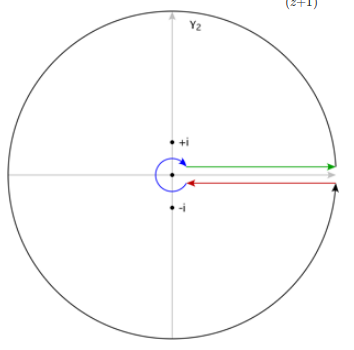
\includegraphics{figures/image_2021-06-09-02-11-59.png}
\caption{image\_2021-06-09-02-11-59}
\end{figure}

Show that outer radius \(R\) and inner radius \(\rho\) circles
contribute zero in the limit by the ML estimate? Compute the residues by
just applying the formula and manually computing derivatives:
\begin{align*}
\mathop{\mathrm{Res}}_{z= \pm i} f(z) 
&= \lim_{z\to \pm i} {\frac{\partial }{\partial z}\,} {\log^2(z) \over (z\pm i)^2} \\
&= \lim_{z\to \pm i} {2\log(z) (z\pm i)^2 - 2(z\pm i)^2 \log^2(z) \over \qty{(z\pm i )^2}^2} \\
&= {
2\log(\pm i)(\pm 2i)^2 - 2(\pm 2i)^2 \log^2(\pm i)
\over {\qty{\pm 2i}}^4 } \\
&=_? {\pi \over 4}\pm {i\pi^2 \over 16}
.\end{align*}

\begin{quote}
See p.4: \url{http://www.math.toronto.edu/mnica/complex1.pdf}
\end{quote}

\end{solution}

\begin{exercise}[Sinc Function]

Show
\begin{align*}
\int_{(0, \infty)} {\sin(x) \over x }\,dx= {\pi \over 2}
.\end{align*}

\end{exercise}

\begin{solution}

Take an indented semicircle. Let \(I\) be the original integral, then
\begin{align*}
I = {1\over 2i} \int_{\mathbb{R}}{e^{iz} - 1 \over z } \,dz
.\end{align*}

\end{solution}

\begin{figure}
\centering
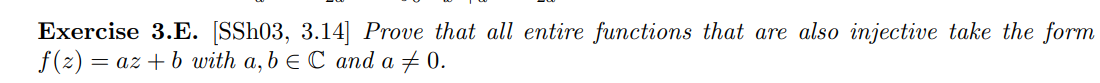
\includegraphics{figures/image_2021-05-17-13-33-55.png}
\caption{image\_2021-05-17-13-33-55}
\end{figure}

\hypertarget{integrals-1}{%
\section{Integrals}\label{integrals-1}}

\href{https://math.mit.edu/~jorloff/18.04/notes/topic9.pdf}{See this
very detailed note}.

\begin{itemize}
\item
  For integrals that decay faster than \(1/z^\alpha, \alpha>1\):
  semicircular contours.

  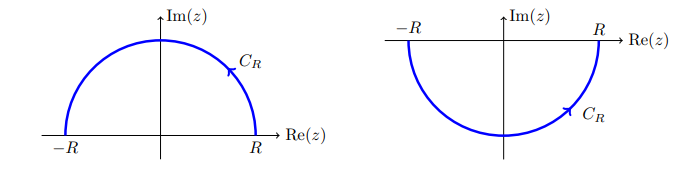
\includegraphics{figures/2021-07-29_18-37-57.png}
\item
  For integrals that decay like \(1/z\): rectangular contours.
\end{itemize}

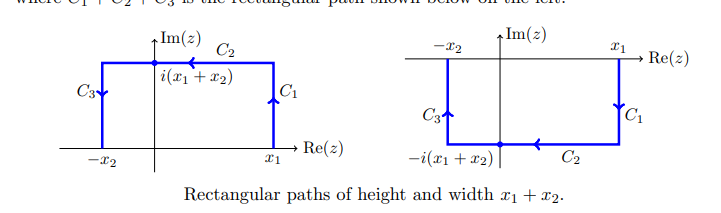
\includegraphics{figures/2021-07-29_18-38-24.png}

\begin{itemize}
\item
  If a trigonometric function is in the numerator, check if
  \(I \approx \Re(\tilde I)\) where \(\tilde I\) replaces cosines/sines
  with \(e^{iz}\).
\item
  For rational functions of \(\cos, \sin\): set
  \(2\cos(z) = z + z^{-1}, 2\sin(z) = z - z^{-1}, \,d\theta= {\,dz\over iz}\)
  to reduce to a residue count in
  \({\left\lvert {z} \right\rvert} \leq 1\).
\end{itemize}

\begin{exercise}[?]

\begin{align*}
\int_{\mathbb{R}}{1 \over (1+x)^2} = {\pi \over 2}
.\end{align*}

Use that \(f(z) \sim 1/z^4\).

\end{exercise}

\begin{solution}

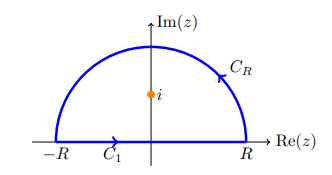
\includegraphics{figures/2021-07-29_18-40-40.png}

\end{solution}

\begin{exercise}[?]

\begin{align*}
\int_{\mathbb{R}}{1 \over x^4 + 1} = {\pi \sqrt{2} \over 2}
.\end{align*}

\end{exercise}

\begin{solution}

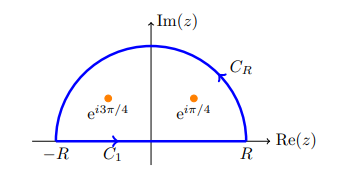
\includegraphics{figures/2021-07-29_18-41-05.png}

\end{solution}

\begin{exercise}[?]

\begin{align*}
\int_{0}^{\infty} \frac{\cos (x)}{x^{2}+b^{2}} d x=\frac{\pi \mathrm{e}^{-b}}{2 b} .
.\end{align*}

\end{exercise}

\begin{solution}

Extend to \(\int_{\mathbb{R}}\) using that \(f\) is even.

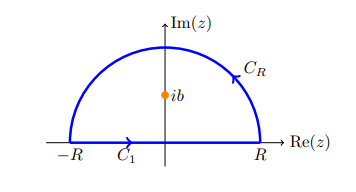
\includegraphics{figures/2021-07-29_18-42-38.png}

\end{solution}

\begin{exercise}[Trigonometric functions]

\begin{align*}
\int_{0}^{2 \pi} \frac{d \theta}{1+a^{2}-2 a \cos (\theta)}
= \begin{cases}\frac{2 \pi}{a^{2}-1} & \text { if }|a|>1 \\ \frac{2 \pi}{1-a^{2}} & \text { if }|a|<1\end{cases}
.\end{align*}

\end{exercise}

\begin{solution}

Write \(2\cos(z) = z + z^{-1}\) on \(S^1\) to get
\begin{align*}
=\int_{|z|=1} \frac{1}{i\left(\left(1+a^{2}\right) z-a\left(z^{2}+1\right)\right)} d z
.\end{align*}

\end{solution}

\hypertarget{branch-cuts}{%
\subsection{Branch Cuts}\label{branch-cuts}}

\begin{exercise}[?]

\begin{align*}
\int_0^\infty {x^{1\over 3} \over 1 + x^2} \,dx= {\pi \over \sqrt 3}
.\end{align*}

\end{exercise}

\begin{solution}

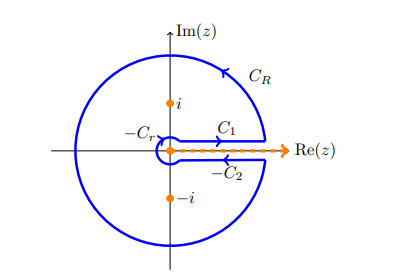
\includegraphics{figures/2021-07-29_18-51-17.png}

\end{solution}

\begin{exercise}[?]

\begin{align*}
\int_{1}^{\infty} \frac{d x}{x \sqrt{x^{2}-1}} = {\pi \over 2}
.\end{align*}

\end{exercise}

\begin{solution}

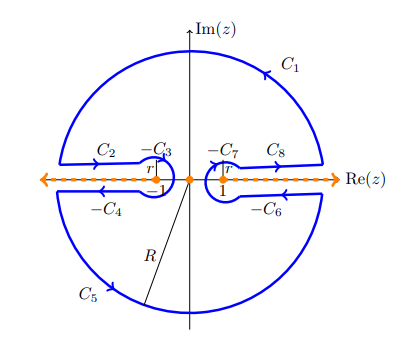
\includegraphics{figures/2021-07-29_18-53-35.png}

\end{solution}

\hypertarget{conformal-maps-linear-fractional-transformations}{%
\section{Conformal Maps / Linear Fractional
Transformations}\label{conformal-maps-linear-fractional-transformations}}

\begin{definition}[Conformal Map / Biholomorphism]

A map \(f\) is \textbf{conformal} on \(\Omega\) iff \(f\) is
complex-differentiable, \(f'(z)\neq 0\) for \(z\in \Omega\), and \(f\)
preserves signed angles (so \(f\) is orientation-preserving). Conformal
implies holomorphic, and a bijective conformal map has conformal inverse
automatically.

A bijective conformal map \(f:U\to V\) \textbf{biholomorphism}, and we
say \(U\) and \(V\) are \textbf{biholomorphic}. Importantly, bijective
holomorphic maps always have holomorphic inverses. Self-biholomorphisms
of a domain \(\Omega\) form a group
\(\mathop{\mathrm{Aut}}_{\mathbb{C}}(\Omega)\).

\end{definition}

\begin{remark}

There is an oft-used weaker condition that \(f'(z) \neq 0\) for any
point. Note that that this condition alone doesn't necessarily imply
\(f\) is holomorphic, since anti-holomorphic maps may have nonzero
derivatives. For example, take
\(f(z) = \mkern 1.5mu\overline{\mkern-1.5muz\mkern-1.5mu}\mkern 1.5mu\),
so \(f(x+iy) = x-iy\) -- this does not satisfy the Cauchy-Riemann
equations.

\end{remark}

\begin{remark}

A bijective holomorphic map automatically has a holomorphic inverse.
This can be weakened: an injective holomorphic map satisfies
\(f'(z) \neq 0\) and \(f ^{-1}\) is well-defined on its range and
holomorphic.

\end{remark}

\begin{definition}[Linear fractional transformation / Mobius transformation]

A map of the following form is a \emph{linear fractional
transformation}:
\begin{align*}  
T(z) = {az + b \over cz + d}
,\end{align*}
where the denominator is assumed to not be a multiple of the numerator.
These have inverses given by
\begin{align*}  
T^{-1}(w) = {dw-b \over -cw + a}
.\end{align*}

\end{definition}

\begin{proposition}[?]

Given any three points \(z_1, z_2, z_3\), the following Möbius
transformation sends them to \(1, 0, \infty\) respectively:
\begin{align*}
T(z) 
&\coloneqq{ (z-z_1) (z_2-z_3) \over (z-z_3) (z_2 - z_1)}
\\
z_1 & \mapsto 0 \\
z_2 & \mapsto 1 \\
z_3 & \mapsto \infty
.\end{align*}
Such a map is sometimes denoted \((z; z_1, z_2, z_3)\). One can use this
to produce a map sending any three points to any other three points:
\begin{align*}
T(z) \coloneqq
(w; w_1, w_2, w_3)^{-1}
\circ
(z; z_1,z_2, z_3)
.\end{align*}

\end{proposition}

\begin{example}[?]

\envlist

\begin{itemize}
\tightlist
\item
  \((z, i, 1, -1): {\mathbb{D}}\to {\mathbb{H}}\)
\item
  \((z, 0, -1, 1): {\mathbb{D}}\cap{\mathbb{H}}\to Q_1\).
\end{itemize}

\end{example}

\begin{theorem}[Cayley Transform]

The fractional linear transformation given by
\(F(z) = {i - z \over i + z}\) maps \({\mathbb{D}}\to {\mathbb{H}}\)
with inverse \(G(w) = i {1-w \over 1 + w}\).

\end{theorem}

\begin{theorem}[Characterization of conformal maps]

Conformal maps \({\mathbb{D}}\to{\mathbb{D}}\) have the form
\begin{align*}
g(z) = \lambda {1-a \over 1 - \mkern 1.5mu\overline{\mkern-1.5mua\mkern-1.5mu}\mkern 1.5mu z}, \quad {\left\lvert {a} \right\rvert} < 1, \quad {\left\lvert {\lambda} \right\rvert} = 1
.\end{align*}

\end{theorem}

\begin{theorem}[Riemann Mapping]

If \(\Omega\) is simply connected, nonempty, and not \({\mathbb{C}}\),
then for every \(z_{0}\in \Omega\) there exists a unique conformal map
\(F:\Omega \to {\mathbb{D}}\) such that \(F(z_{0}) = 0\) and
\(F'(z_{0}) > 0\).

Thus any two such sets \(\Omega_{1}, \Omega_{2}\) are conformally
equivalent.

\end{theorem}

\hypertarget{by-type}{%
\subsection{By Type}\label{by-type}}

\begin{remark}[Notation]

\begin{longtable}[]{@{}
  >{\raggedright\arraybackslash}p{(\columnwidth - 2\tabcolsep) * \real{0.64}}
  >{\raggedright\arraybackslash}p{(\columnwidth - 2\tabcolsep) * \real{0.35}}@{}}
\toprule
Notation & Definition \\
\midrule
\endhead
\({\mathbb{D}}\coloneqq\left\{{z {~\mathrel{\Big|}~}{\left\lvert {z} \right\rvert} \leq 1}\right\}\)
& The unit disc \\
\({\mathbb{H}}\coloneqq\left\{{x+iy {~\mathrel{\Big|}~}y > 0}\right\}\)
& The upper half-plane \\
\(X_{1\over 2}\) & A ``half version of \(X\)'', see examples \\
\({\mathbb{H}}_{1\over 2}\) & The first quadrant \\
\({\mathbb{D}}_{1\over 2}\) & The portion of the first quadrant inside
the unit disc \\
\(L \coloneqq\left\{{x + iy {~\mathrel{\Big|}~}x\in {\mathbb{R}},\, 0<y<\pi}\right\}\)
& The horizontal strip \\
\bottomrule
\end{longtable}

\end{remark}

\begin{theorem}[Classification of Conformal Maps]

There are 8 major types of conformal maps:

\begin{longtable}[]{@{}
  >{\raggedright\arraybackslash}p{(\columnwidth - 2\tabcolsep) * \real{0.62}}
  >{\raggedright\arraybackslash}p{(\columnwidth - 2\tabcolsep) * \real{0.37}}@{}}
\toprule
Type/Domains & Formula \\
\midrule
\endhead
Translation & \(z\mapsto z + h\) \\
Dilation & \(z\mapsto cz\) \\
Rotation & \(z\mapsto e^{i\theta}\) \\
Sectors to sectors & \(z\mapsto z^n\) \\
\({\mathbb{D}}_{1\over 2} \to {\mathbb{H}}_{1\over 2}\), the first
quadrant & \(z\mapsto {1+z \over 1-z}\) \\
\({\mathbb{H}}\to S\) & \(z\mapsto \log(z)\) \\
\({\mathbb{D}}_{1\over 2} \to L_{1\over 2}\) & \(z\mapsto \log(z)\) \\
\(S_{1\over 2} \to {\mathbb{D}}_{1\over 2}\) & \(z\mapsto e^{iz}\) \\
\({\mathbb{D}}_{1\over 2} \to {\mathbb{H}}\) &
\(z\mapsto {1\over 2}\qty{z + {1\over z}}\) \\
\(L_{1\over 2} \to {\mathbb{H}}\) & \(z\mapsto \sin(z)\) \\
\bottomrule
\end{longtable}

\end{theorem}

\todo[inline]{Pictures!}

\begin{proposition}[Half-plane to Disc]

\begin{align*}
F: {\mathbb{H}}^\circ &\rightleftharpoons{\mathbb{D}}^\circ \\
\left\{{z{~\mathrel{\Big|}~}\Im(z) > 0 }\right\} &\rightleftharpoons\left\{{w{~\mathrel{\Big|}~}{\left\lvert {w} \right\rvert} < 1 }\right\} \\
z &\mapsto {i-z \over i+z} \\
i \qty{1-w \over 1+w} &\mapsfrom w
.\end{align*}

\textbf{Boundary behavior:}

\begin{itemize}
\tightlist
\item
  This maps \({\mathbb{R}}\to {{\partial}}{\mathbb{D}}\), where
  \(F(\infty) = -1\), and as \(x\in {\mathbb{R}}\) ranges from
  \(-\infty\to\infty\), \(F(x)\) travels from \(z=-1\) counter-clockwise
  through \(S^1\) (starting at \(z=-1\) and moving through the lower
  half first).
\end{itemize}

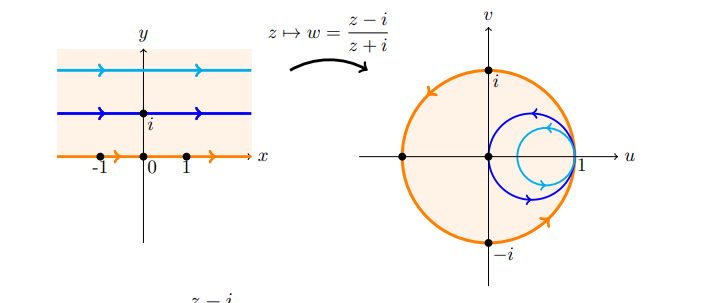
\includegraphics{figures/2021-07-29_19-02-54.png}

So this extends to a map \({\mathbb{H}}\to {\mathbb{D}}\).

\begin{quote}
Mnemonic: every \(z\in {\mathbb{H}}\) is closer to \(i\) than \(-i\).
\end{quote}

\end{proposition}

\begin{remark}

Some write a similar map:
\begin{align*}
{\mathbb{H}}^\circ &\to {\mathbb{D}}^\circ \\
z &\mapsto {z-i \over z+i}
.\end{align*}
This is just a composition of the above map with the flip
\(z\mapsto -z\):
\begin{align*}
- {i-z \over i + z} = {z-i \over i+z} = {z-i \over z+i}
.\end{align*}

\end{remark}

\begin{proposition}[Right half-plane to Disc]

\begin{align*}
{\mathbb{H}}_{R} &\rightleftharpoons{\mathbb{D}}\\
\left\{{ z {~\mathrel{\Big|}~}\Re(z) > 0 }\right\} &\rightleftharpoons\left\{{ w {~\mathrel{\Big|}~}{\left\lvert {w} \right\rvert} < 1 }\right\} \\
z &\mapsto {1-z \over 1+z} \\
{1-w\over 1+w} &\mapsfrom w
.\end{align*}

Just map the \emph{right} half-plane \({\mathbb{H}}_R\) to the disc
\({\mathbb{D}}\) by precomposing with a rotation \(e^{i\pi/2} = i\):
\begin{align*}
{\mathbb{H}}_{R} \to {\mathbb{H}}&\to {\mathbb{D}}\\
z \mapsto iz &\mapsto {i- (iz) \over i + (iz)} = {i(1-z) \over i(1+z) } = {1-z \over 1+z}
.\end{align*}

This can easily be inverted:
\begin{align*}
&\quad w = {1+z \over 1+z} \\
&\implies -(1-w) + z(w+1) = 0 \\
&\implies z = {1-w \over 1+w}
.\end{align*}

\textbf{Boundary behavior}: Just a rotated version of
\({\mathbb{H}}\to {\mathbb{D}}\)!

\begin{quote}
Mnemonic: every \(z\in {\mathbb{H}}_R\) is closed to 1 than \(-1\).
\end{quote}

\end{proposition}

\begin{proposition}[Sector to sector]

For \(0 < \alpha < 2\):
\begin{align*}
F_\alpha: S_{\pi \over \alpha }^\circ &\rightleftharpoons S_{\pi}^\circ = {\mathbb{H}}^\circ \\
\left\{{z{~\mathrel{\Big|}~}0 < \operatorname{Arg}(z) < {\pi\over \alpha} }\right\} &\rightleftharpoons\left\{{w{~\mathrel{\Big|}~}0 < \operatorname{Arg}(w) < \pi }\right\} \\
z &\mapsto z^\alpha \\
w^{1\over \alpha} &\mapsfrom w
.\end{align*}
Note that if you look at the image of \({\mathbb{H}}\) under
\(z\mapsto z^{\alpha}\), you get
\begin{align*}
\left\{{z {~\mathrel{\Big|}~}0 < \operatorname{Arg}(z) < \pi }\right\} &\rightleftharpoons\left\{{0 < \operatorname{Arg}(w) < \alpha \pi }\right\} 
.\end{align*}
For the inverse, choose a branch cut of \(\log\) deleting the negative
real axis, or more generally fix \(0 < \arg w < \alpha \pi\).

\textbf{Boundary behavior:}

\begin{itemize}
\tightlist
\item
  As \(x\) travels from \(-\infty\to 0\), \(F_\alpha(x)\) travels
  \emph{away} from infinity along the ray \(\theta = \alpha \pi\), so
  \(L = \left\{{ e^{t \alpha \pi } {~\mathrel{\Big|}~}t\in (0, \infty) }\right\}\),
  from \(\infty\to 0\).
\item
  As \(x\) travels from \(0\to \infty\), \(F_\alpha(x)\) travels from
  \(0\to \infty\) along \({\mathbb{R}}\).
\end{itemize}

\end{proposition}

\begin{proposition}[Sector to Disc]

The unmotivated formula first:
\begin{align*}
F: S_{\alpha} &\to {\mathbb{D}}\\ \\
\left\{{ z {~\mathrel{\Big|}~}0 < \operatorname{Arg}(z) < \alpha }\right\} &\rightleftharpoons\left\{{ w {~\mathrel{\Big|}~}{\left\lvert {w} \right\rvert} < 1 }\right\} \\
z &\rightleftharpoons{z^{\pi\over \alpha} - i \over z^{\pi\over\alpha} + i}
.\end{align*}

Idea: compose some known functions.

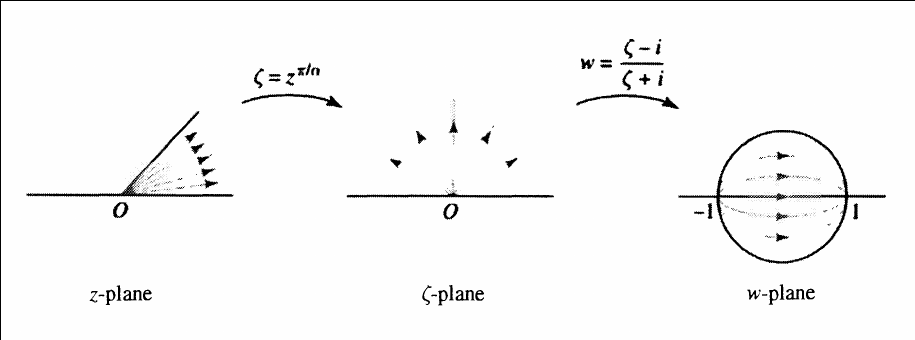
\includegraphics{figures/image_2020-07-22-13-22-46.png}

\begin{align*}
S_{\alpha} &\to S_{\pi} = {\mathbb{H}}\to {\mathbb{D}}\\
z &\mapsto z^{\pi \over \alpha} \mapsto {z-i\over z+i}\Big|_{z= z^{\pi\over \alpha}}
.\end{align*}

\end{proposition}

\begin{proposition}[Upper half-disc to first quadrant]

\begin{align*}
\left\{{ z {~\mathrel{\Big|}~}{\left\lvert {z} \right\rvert} < 1,\, \Im(z) > 0 }\right\} &\rightleftharpoons\left\{{ w {~\mathrel{\Big|}~}\Re(w)>0,\, \Im(w) > 0}\right\}  \\
z &\mapsto {1+z \over 1-z} \\
{w-1\over w+1} &\mapsfrom w
.\end{align*}

\begin{itemize}
\tightlist
\item
  Why this lands in the first quadrant:

  \begin{itemize}
  \tightlist
  \item
    Use that squares are non-negative and
    \(z=x+iy\in {\mathbb{D}}\implies x^2 + y^2 < 1\):
    \begin{align*}
    f(z)=\frac{1-\left(x^{2}+y^{2}\right)}{(1-x)^{2}+y^{2}}+i \frac{2 y}{(1-x)^{2}+y^{2}}
    .\end{align*}
  \end{itemize}
\item
  Why the inverse lands in the unit disc:

  \begin{itemize}
  \tightlist
  \item
    For \(w\) in Q1, the distance from \(w\) to 1 is smaller than from
    \(w\) to \(-1\).
  \item
    Check that if \(w=u+iv\) where \(u, v>0\), the imaginary part of the
    image is positive:
  \end{itemize}
\end{itemize}

\begin{align*}
{w-1 \over w+1} 
&= { (w-1) \mkern 1.5mu\overline{\mkern-1.5mu(w+1)\mkern-1.5mu}\mkern 1.5mu \over {\left\lvert {w+1} \right\rvert}^2}\\
&={ \qty{u-1 + iv} \qty{u+1-iv} \over (u+1)^2 + v^2 } \\
&= {u^2 + v^2 + 1 \over (u+1)^2 + v^2}
+ i\qty{ 2v \over (u+1)^2 + v^2}
.\end{align*}

\textbf{Boundary behavior}:

\begin{itemize}
\item
  On the upper half circle
  \(\left\{{ e^{it } {~\mathrel{\Big|}~}t\in (0, \pi) }\right\}\), write
  \begin{align*}
  f(z)=\frac{1+e^{i \theta}}{1-e^{i \theta}}=\frac{e^{-i \theta / 2}+e^{i \theta / 2}}{e^{-i \theta / 2}-e^{i \theta / 2}}=\frac{i}{\tan (\theta / 2)}
  ,\end{align*}
  so as \(t\) ranges \(0\to \pi\) we have \(f(z)\) ranging from
  \(0\to i\infty\) along the imaginary axis.
\item
  As \(x\) ranges from \(-1\to 1\) in \({\mathbb{R}}\), \(f(z)\) ranges
  from \(0\to \infty\) with \(f(0) = 1\).
\end{itemize}

\end{proposition}

\begin{proposition}[Log: Upper half-plane to horizontal strip]

\begin{align*}
{\mathbb{H}}&\rightleftharpoons{\mathbb{R}}\times(0, \pi) \\
\left\{{ z {~\mathrel{\Big|}~}\Im(z) > 0 }\right\} &\rightleftharpoons\left\{{ w {~\mathrel{\Big|}~}\Im(z) \in (0, \pi ) }\right\} \\
z &\mapsto \log(z) \\
e^w &\mapsfrom w
.\end{align*}

\begin{itemize}
\tightlist
\item
  Why this lands in a strip: use that \(\arg(z) \in (0, \pi)\) and
  \(\log(z) = {\left\lvert {z} \right\rvert} + i\arg(z)\).
\end{itemize}

\textbf{Boundary behavior}:

\begin{itemize}
\tightlist
\item
  As \(x\) travels from \(-\infty \to 0\), \(F(x)\) travels horizontally
  from \(\infty + i\pi\) to \(-\infty + i\pi\).
\item
  As \(x\) travels from \(o\to \infty\), \(F(x)\) travels from
  \(-\infty\to\infty\) in \({\mathbb{R}}\).
\end{itemize}

\end{proposition}

\begin{remark}

This extends to a function
\({\mathbb{C}}\setminus{\mathbb{R}}^{\leq 0} \to {\mathbb{R}}\times(-\pi, \pi)\).
Circles of radius \(R\) are mapped to vertical line segments connecting
\(\ln(R) + i\pi\) to \(\ln(R) - i\pi\), and rays are mapped to
horizontal lines.

\end{remark}

\begin{remark}

One can find other specific images of the logarithm:
\begin{align*}
\left\{{ z {~\mathrel{\Big|}~}{\left\lvert {z} \right\rvert} < 1,\, \Im(z) > 0 }\right\} &\rightleftharpoons{\mathbb{R}}^{<0} \times(0, \pi ) \\
\left\{{ z {~\mathrel{\Big|}~}{\left\lvert {z} \right\rvert} > 1,\, \Im(z) > 0 }\right\} &\rightleftharpoons{\mathbb{R}}^{>0} \times(0, \pi ) \\
.\end{align*}

For the upper half-disc to the negative horizontal half-strip: - As
\(x\) travels \(0\to 1\) in \({\mathbb{R}}\), \(\log(x)\) travels from
\(-\infty\to 0\). - As \(x\) travels from \(-1\) to \(1\) along
\(S^1\cap{\mathbb{H}}\), \(\log(x)\) travels from \(0\to i\pi\)
vertically. - As \(x\) travels from \(-1\to 0\), \(\log(x)\) travels
from \(0+i\pi\to i-\infty+i\pi\) along the top of the strip.

\end{remark}

\begin{proposition}[Half-discs to half strips]

\begin{align*}
F: (-{\pi\over 2}, {\pi \over 2}) \times{\mathbb{R}}^{>0} &\to {\mathbb{D}}\cap{\mathbb{H}}\\
z &\mapsto e^{iz} \\
{\log(w) \over i}? &\mapsfrom w
.\end{align*}

This uses that \(e^{iz} = e^{-\Im(z)} e^{i \Re(z)}\).

\textbf{Boundary behavior}:

\end{proposition}

\begin{proposition}[Half-disc to upper half-plane]

\begin{align*}
F: ? &\rightleftharpoons? \\
z & \mapsto -{1\over 2}\qty{z + z^{-1}} \\
.\end{align*}

\end{proposition}

\begin{proposition}[Upper half-plane to vertical half-strip]

\begin{align*}
? &\rightleftharpoons? \\
z &\mapsto \sin(z) \\
.\end{align*}

\end{proposition}

\hypertarget{exercises-4}{%
\subsection{Exercises}\label{exercises-4}}

\begin{exercise}[?]

Find a conformal map from the upper half-disc to the upper half-plane.

\end{exercise}

\begin{solution}

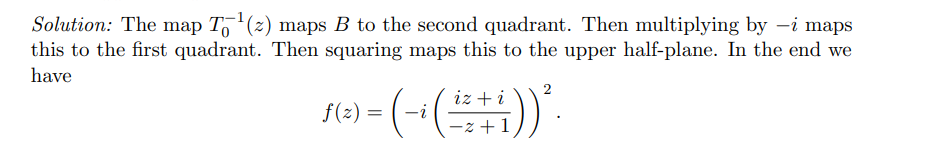
\includegraphics{figures/2021-07-29_19-26-39.png}

\end{solution}

\hypertarget{schwarz-reflection}{%
\section{Schwarz Reflection}\label{schwarz-reflection}}

\hypertarget{schwarz}{%
\subsection{Schwarz}\label{schwarz}}

\begin{theorem}[Schwarz Lemma]\label{SchwarzzLemma}

If \(f: {\mathbb{D}}\to {\mathbb{D}}\) is holomorphic with \(f(0) = 0\),
then

\begin{enumerate}
\def\labelenumi{\arabic{enumi}.}
\tightlist
\item
  \({\left\lvert {f(z)} \right\rvert} \leq {\left\lvert {z} \right\rvert}\)
  for all \(z\in {\mathbb{D}}\)
\item
  \({\left\lvert {f'(0)} \right\rvert} \leq 1\).
\end{enumerate}

Moreover, if

\begin{itemize}
\tightlist
\item
  \({\left\lvert {f(z_0)} \right\rvert} = {\left\lvert {z_0} \right\rvert}\)
  for any \(z_0\in {\mathbb{D}}\), or
\item
  \({\left\lvert {f'(0)} \right\rvert} = 1\),
\end{itemize}

then \(f\) is a rotation.

\end{theorem}

\begin{proof}[?]

Apply the maximum modulus principle to \(f(z)/z\).

\end{proof}

\begin{exercise}[?]

Show that
\(\mathop{\mathrm{Aut}}_{\mathbb{C}}({\mathbb{C}}) = \left\{{ z \mapsto az+b{~\mathrel{\Big|}~}a\in {\mathbb{C}}^{\times}, b\in {\mathbb{C}}}\right\}\).

\end{exercise}

\begin{theorem}[Biholomorphisms of the disc]

\begin{align*}
\mathop{\mathrm{Aut}}_{\mathbb{C}}({\mathbb{D}}) = \left\{{ z\mapsto e^{i\theta} \qty{\alpha - z \over 1 - \mkern 1.5mu\overline{\mkern-1.5mu\alpha\mkern-1.5mu}\mkern 1.5mu z} }\right\}
.\end{align*}

\end{theorem}

\begin{proof}[?]

Schwarz lemma.

\end{proof}

\begin{theorem}[?]

\begin{align*}
\mathop{\mathrm{Aut}}_{\mathbb{C}}({\mathbb{H}}) = \left\{{ z \mapsto {az+b \over cz+d} {~\mathrel{\Big|}~}a,b,c,d\in {\mathbb{C}}, ad-bc=1 }\right\} \cong{\operatorname{PSL}}_2({\mathbb{R}})
.\end{align*}

\end{theorem}

\todo[inline]{?}

\hypertarget{schwarz-lemma}{%
\section{Schwarz Lemma}\label{schwarz-lemma}}

\todo[inline]{?}

\todo[inline]{Montel's theorem}

\todo[inline]{Normal families}

\todo[inline]{Schwarz lemma}

\todo[inline]{Equicontinuity}

\hypertarget{unsorted-theorems}{%
\section{Unsorted Theorems}\label{unsorted-theorems}}

\begin{theorem}[Riemann's Removable Singularity Theorem]

If \(f\) is holomorphic on \(\Omega\) except possibly at \(z_0\) and
\(f\) is bounded on \(\Omega\setminus\left\{{z_0}\right\}\), then
\(z_0\) is a removable singularity.

\end{theorem}

\begin{theorem}[Little Picard]

If \(f:{\mathbb{C}}\to {\mathbb{C}}\) is entire and nonconstant, then
\(\operatorname{im}(f)\) is either \({\mathbb{C}}\) or
\({\mathbb{C}}\setminus\left\{{z_0}\right\}\) for some point \(z_0\).

\end{theorem}

\todo{???}

\begin{corollary}

The ring of holomorphic functions on a domain in \({\mathbb{C}}\) has no
zero divisors.

\end{corollary}

\begin{proof}

???

\end{proof}

\todo[inline]{Find the proof!}

Morera

\begin{proposition}[Bounded Complex Analytic Functions form a Banach Space]

For \(\Omega\subseteq{\mathbb{C}}\), show that
\(A({\mathbb{C}})\coloneqq\left\{{f: \Omega \to {\mathbb{C}}{~\mathrel{\Big|}~}f\text{ is bounded}}\right\}\)
is a Banach space.

\end{proposition}

\begin{proof}

?

\begin{quote}
Apply Morera's Theorem and Cauchy's Theorem
\end{quote}

\end{proof}

\hypertarget{proofs-of-the-fundamental-theorem-of-algebra}{%
\section{Proofs of the Fundamental Theorem of
Algebra}\label{proofs-of-the-fundamental-theorem-of-algebra}}

\hypertarget{argument-principle-1}{%
\subsubsection{Argument Principle}\label{argument-principle-1}}

\begin{proof}[using the argument principle]

\envlist

\begin{itemize}
\tightlist
\item
  Let \(P(z) = a_nz^n + \cdots + a_0\) and \(g(z) = P'(z)/P(z)\), note
  \(P\) is holomorphic
\item
  Since
  \(\lim_{{\left\lvert {z} \right\rvert} \to \infty} P(z) = \infty\),
  there exist an \(R>0\) such that \(P\) has no roots in
  \(\left\{{{\left\lvert {z} \right\rvert} \geq R}\right\}\).
\item
  Apply the argument principle:
  \begin{align*}     N(0) = {1\over 2\pi i} \oint_{{\left\lvert {\xi} \right\rvert} = R} g(\xi) \,d\xi     .\end{align*}
\item
  Check that
  \(\lim_{{\left\lvert {z\to \infty} \right\rvert}}zg(z) = n\), so \(g\)
  has a simple pole at \(\infty\)
\item
  Then \(g\) has a Laurent series
  \({n\over z} + {c_2 \over z^2} + \cdots\)
\item
  Integrate term-by-term to get \(N(0) = n\).
\end{itemize}

\end{proof}

\hypertarget{rouches-theorem}{%
\subsubsection{Rouche's Theorem}\label{rouches-theorem}}

\begin{proof}[using Rouche's theorem]

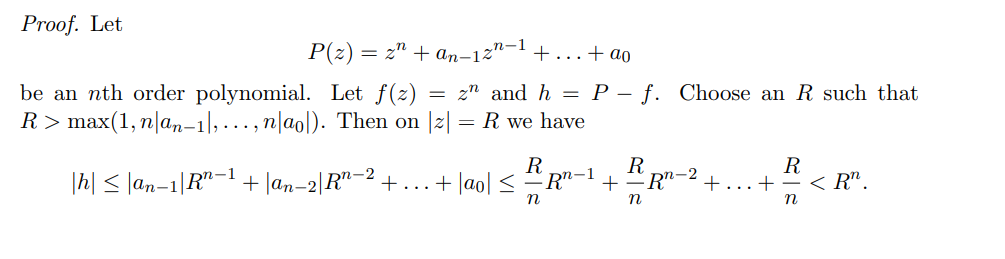
\includegraphics{figures/2021-07-29_20-41-18.png}
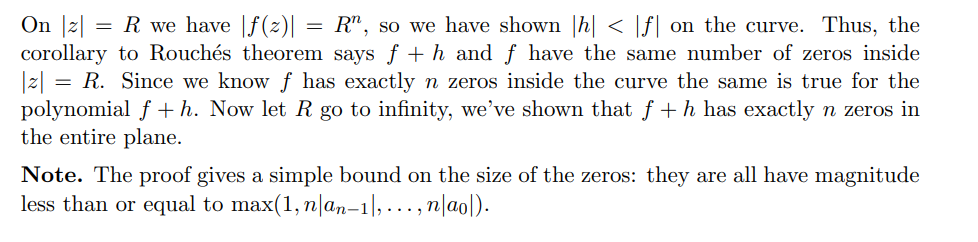
\includegraphics{figures/2021-07-29_20-41-29.png}

\begin{itemize}
\tightlist
\item
  Let \(P(z) = a_nz^n + \cdots + a_0\)
\item
  Set \(f(z) = a_n z^n\) and
  \(g(z) = P(z) - f(z) = a_{n-1}z^{n-1} + \cdots + a_0\), so
  \(f+g = P\).
\item
  Choose
  \(R > \max\qty{ { {\left\lvert {a_{n-1}} \right\rvert} + \cdots + {\left\lvert {a_0} \right\rvert} \over {\left\lvert {a_n} \right\rvert} }, 1}\),
  then
\end{itemize}

\begin{align*} |g(z)|  &\coloneqq|a_{n-1}z^{n-1} + \cdots + a_1 z + a_0 | \\ &\leq |a_{n-1}z^{n-1}| + \cdots + |a_1 z| + |a_0 | \quad\text{by the triangle inequality} \\ &= |a_{n-1}|\cdot |z^{n-1}| + \cdots + |a_1|\cdot| z| + |a_0 | \\ &=  |a_{n-1}|\cdot R^{n-1} + \cdots + |a_1| R + |a_0 | \\ &\leq |a_{n-1}|\cdot R^{n-1}+|a_{n-2}|\cdot R^{n-1} + \cdots + |a_1| \cdot R^{n-1} + |a_0 |\cdot R^{n-1} \quad\text{since } R>1 \implies R^{a+b} \geq R^a \\ &= R^{n-1} \left( |a_{n-1}| + |a_{n-2}| + \cdots + |a_1| + |a_0| \right) \\ &\leq R^{n-1} \left( |a_n|\cdot R \right) \quad\text{by choice of } R   \\ &= R^{n} |a_n| \\ &= |a_n z^n| \\ &\coloneqq|f(z)| \end{align*}

\begin{itemize}
\tightlist
\item
  Then \(a_n z^n\) has \(n\) zeros in
  \({\left\lvert {z} \right\rvert} < R\), so \(f+g\) also has \(n\)
  zeros.
\end{itemize}

\end{proof}

\hypertarget{liouvilles-theorem}{%
\subsubsection{Liouville's Theorem}\label{liouvilles-theorem}}

\begin{proof}[using Liouville's theorem]

\envlist

\begin{itemize}
\tightlist
\item
  Suppose \(p\) is nonconstant and has no roots, then \({1\over p}\) is
  entire. We will show it is also bounded and thus constant, a
  contradiction.
\item
  Write
  \(p(z) = z^n \left(a_n + \frac{a_{n-1}}{z}+\dots+\frac{a_{0}}{z^{n}}\right)\)
\item
  Outside a disc:

  \begin{itemize}
  \tightlist
  \item
    Note that \(p(z) \overset{z\to \infty }\to \infty\). so there exists
    an \(R\) large enough such that
    \({\left\lvert {p(z)} \right\rvert} \geq {1\over A}\) for any fixed
    chosen constant \(A\).
  \item
    Then \({\left\lvert { 1/p(z)} \right\rvert} \leq A\) outside of
    \({\left\lvert {z} \right\rvert} >R\), i.e.~\(1/p(z)\) is bounded
    there.
  \end{itemize}
\item
  Inside a disc:

  \begin{itemize}
  \tightlist
  \item
    \(p\) is continuous with no roots and thus must be bounded below on
    \({\left\lvert {z} \right\rvert} < R\).
  \item
    \(p\) is entire and thus continuous, and since
    \(\mkern 1.5mu\overline{\mkern-1.5muD\mkern-1.5mu}\mkern 1.5mu_r(0)\)
    is a compact set, \(p\) achieves a min \(A\) there
  \item
    Set \(C \coloneqq\min(A, B)\), then
    \({\left\lvert {p(z)} \right\rvert} \geq C\) on all of
    \({\mathbb{C}}\) and thus
    \({\left\lvert {1/p(z)} \right\rvert} \leq C\) everywhere.
  \item
    So \(1/p(z)\) is bounded an entire and thus constant by Liouville's
    theorem -- but this forces \(p\) to be constant. \(\contradiction\)
  \end{itemize}
\end{itemize}

\end{proof}

\hypertarget{open-mapping-theorem}{%
\subsubsection{Open Mapping Theorem}\label{open-mapping-theorem}}

\begin{proof}[using the Open Mapping theorem]

\envlist

\begin{itemize}
\tightlist
\item
  \(p\) induces a continuous map \({\mathbb{CP}}^1 \to {\mathbb{CP}}^1\)
\item
  The continuous image of compact space is compact;
\item
  Since the codomain is Hausdorff space, the image is closed.
\item
  \(p\) is holomorphic and non-constant, so by the Open Mapping Theorem,
  the image is open.
\item
  Thus the image is clopen in \({\mathbb{CP}}^1\).
\item
  The image is nonempty, since \(p(1) = \sum a_i \in {\mathbb{C}}\)
\item
  \({\mathbb{CP}}^1\) is connected
\item
  But the only nonempty clopen subset of a connected space is the entire
  space.
\item
  So \(p\) is surjective, and \(p^{-1}(0)\) is nonempty.
\item
  So \(p\) has a root.
\end{itemize}

\end{proof}

\hypertarget{generalized-liouville}{%
\subsubsection{Generalized Liouville}\label{generalized-liouville}}

\begin{theorem}[Generalized Liouville]

If \(X\) is a compact complex manifold, any holomorphic
\(f:X\to {\mathbb{C}}\) is constant.

\end{theorem}

\begin{lemma}[?]

If \(f:X\to Y\) is a nonconstant holomorphic map between Riemann
surfaces with \(X\) compact, then

\begin{itemize}
\tightlist
\item
  \(f\) must be surjective,
\item
  \(Y\) must be compact,
\item
  \(f^{-1}(q)\) is finite for all \(q\in Y\),
\item
  The branch and ramification loci consist of finitely many points.
\end{itemize}

\end{lemma}

\begin{proof}[of FTA, using Generalized Liouville]

Given a nonconstant \(p\in {\mathbb{C}}[x]\), regard it as a function
\(p: {\mathbb{P}}^1({\mathbb{C}}) \to {\mathbb{P}}^1({\mathbb{C}})\) by
extending so that \(p(\infty) = \infty\). Since \(p\) is nonconstant, by
the lemma \(p\) is surjective, so there exists some \(x\neq \infty\) in
\({\mathbb{P}}^1({\mathbb{C}})\) with \(p(x) = 0\).

\end{proof}

\hypertarget{appendix}{%
\section{Appendix}\label{appendix}}

\begin{definition}[Gamma function]

\begin{align*}
\Gamma(z) = \int_0^\infty t^{z-1}e^{-t} \,dt
.\end{align*}

\end{definition}

\begin{remark}

Some interesting properties of \(\Gamma\): \(\Gamma(z+1) = z\Gamma(z)\)
and has simple poles at \(z=0,-1,-2,\cdots\) with residues
\(\mathop{\mathrm{Res}}_{z=-m} \Gamma(z) = (-1)^m/m!\). There is also a
factorization
\begin{align*}
\Gamma(z) = {1 \over ze^{\gamma z} \prod_{n=1}^\infty \qty{1 + {z\over n}}e^{-z\over n} }
\end{align*}
where
\(\gamma \coloneqq\lim_{N\to\infty } \sum_{n=1^N} {1\over n} - \log(N)\)

\begin{align*}
\Gamma(z) \Gamma(1-z) = {\pi \over \sin(\pi z)}
,\end{align*}
which yields a product factorization for \(\sin(\pi z)\).

\({\mathcal{L}}(t^{z-1}, s=1) = \Gamma(z)\) and
\({\mathcal{L}}(t^n, s=1) = \Gamma(n+1)\).

\end{remark}

\begin{theorem}[Uniformization]

Every Riemann surface \(S\) is the quotient of a free proper holomorphic
action of a group \(G\) on the universal cover \(\tilde S\) of \(S\), so
\(S\cong \tilde S/G\) is a biholomorphism. Moreover, \(\tilde S\) is
biholomorphic to either

\begin{itemize}
\tightlist
\item
  \({\mathbb{CP}}^1\)
\item
  \({\mathbb{C}}\)
\item
  \({\mathbb{D}}\)
\end{itemize}

\end{theorem}

\hypertarget{misc-basic-algebra}{%
\subsection{Misc Basic Algebra}\label{misc-basic-algebra}}

\begin{fact}[Standard forms of conic sections]

\envlist

\begin{itemize}
\tightlist
\item
  Circle: \(x^2 + y^2 = r^2\)
\item
  Ellipse: \(\qty{\frac x a}^2 + \qty{\frac y b}^2 = 1\)
\item
  Hyperbola: \(\qty{\frac x a}^2 - \qty{\frac y b}^2 = 1\)

  \begin{itemize}
  \tightlist
  \item
    Rectangular Hyperbola: \(xy = \frac{c^2}{2}\).
  \end{itemize}
\item
  Parabola: \(-4ax + y^2 = 0\).
\end{itemize}

Mnemonic: Write \(f(x, y) = Ax^2 + Bxy + Cy^2 + \cdots\), then consider
the discriminant \(\Delta = B^2 - 4AC\):

\begin{itemize}
\tightlist
\item
  \(\Delta < 0 \iff\) ellipse

  \begin{itemize}
  \tightlist
  \item
    \(\Delta < 0\) and \(A=C, B=0 \iff\) circle
  \end{itemize}
\item
  \(\Delta = 0 \iff\) parabola
\item
  \(\Delta > 0 \iff\) hyperbola
\end{itemize}

\end{fact}

\begin{fact}[Completing the square]

\begin{align*}
x^2 - bx = (x - s)^2 - s^2 \quad\text{where} s = \frac{b}{2} \\
x^2 + bx = (x + s)^2 - s^2 \quad\text{where} s = \frac{b}{2}
.\end{align*}

\end{fact}

\begin{fact}

The sum of the interior angles of an \(n{\hbox{-}}\)gon is \((n-2)\pi\),
where each angle is \(\frac{n-2}{n}\pi\).

\end{fact}

\begin{definition}[The Dirichlet Problem]

Given a bounded piecewise continuous function \(u:S^1\to {\mathbb{R}}\),
is there a unique extension to a continuous harmonic function
\(\tilde u: {\mathbb{D}}\to {\mathbb{R}}\)?

\end{definition}

\begin{remark}

More generally, this is a boundary value problem for a region where the
\emph{values} of the function on the boundary are given. Compare to
prescribing conditions on the normal vector on the boundary, which would
be a Neumann BVP. Why these show up: a harmonic function on a simply
connected region has a harmonic conjugate, and solutions of BVPs are
always analytic functions with harmonic real/imaginary parts.

\end{remark}

\begin{example}[Dirichlet problem on the strip]

See section 27, example 1 in Brown and Churchill. On the strip
\((x, y)\in (0, \pi) \times(0, \infty)\), set up the BVP for temperature
on a thin plate with no sinks/sources:
\begin{align*}
\Delta T = 0 && T(0, y) = 0,\, T(\pi, y) = 0 \,\,\forall y \\ \\
T(x, 0) = \sin(x) && T(x, y) \overset{y\to\infty}\longrightarrow 0
.\end{align*}

Then the following function is harmonic on \({\mathbb{R}}^2\) and
satisfies that Dirichlet problem:
\begin{align*}
T(x ,y) = e^{-y} \sin(x) = \Re(-ie^{iz}) = \Im(e^{iz})
.\end{align*}

\end{example}

\begin{exercise}[?]

Show that there is no continuous square root function defined on all of
\({\mathbb{C}}\).

\end{exercise}

\begin{solution}

Suppose \(f(z)^2 = z\). Then \(f\) is a section to the covering map
\begin{align*}
p: {\mathbb{C}}^{\times}&\to {\mathbb{C}}^{\times}\\
z & \mapsto z^2
,\end{align*}
so \(p\circ f = \operatorname{id}\). Using
\(\pi_1({\mathbb{C}}^{\times}) = {\mathbb{Z}}\), the induced maps are
\(p_*(1) = 2\) and \(f_*(1) = n\) for some \(n\in {\mathbb{Z}}\). But
then \(p_* \circ f_*\) is multiplication by \(2n\), contradicting
\(p_* \circ f_* = \operatorname{id}\) by functoriality.

\end{solution}

\begin{remark}

\begin{align*}
\widehat{f}(\xi) \coloneqq{\mathcal{L}}(f, i\xi) \coloneqq\int_{\mathbb{R}}f(x) e^{-i\xi x} \,dx
.\end{align*}

\end{remark}

Basics

\begin{itemize}
\tightlist
\item
  Show that \({1\over z} \sum_{k=1}^\infty {z^k \over k}\) converges on
  \(S^1 \setminus\left\{{1}\right\}\) using summation by parts.
\item
  Show that any power series is continuous on its domain of convergence.
\item
  Show that a uniform limit of continuous functions is continuous.
\end{itemize}

??

\begin{itemize}
\item
  Show that if \(f\) is holomorphic on \({\mathbb{D}}\) then \(f\) has a
  power series expansion that converges uniformly on every compact
  \(K\subset {\mathbb{D}}\).
\item
  Show that any holomorphic function \(f\) can be uniformly approximated
  by polynomials.
\item
  Show that if \(f\) is holomorphic on a connected region \(\Omega\) and
  \(f'\equiv 0\) on \(\Omega\), then \(f\) is constant on \(\Omega\).
\item
  Show that if \({\left\lvert {f} \right\rvert} = 0\) on
  \({{\partial}}\Omega\) then either \(f\) is constant or \(f\) has a
  zero in \(\Omega\).
\item
  Show that if \(\left\{{f_n}\right\}\) is a sequence of holomorphic
  functions converging uniformly to a function \(f\) on every compact
  subset of \(\Omega\), then \(f\) is holomorphic on \(\Omega\) and
  \(\left\{{f_n'}\right\}\) converges uniformly to \(f'\) on every such
  compact subset.
\item
  Show that if each \(f_n\) is holomorphic on \(\Omega\) and
  \(F \coloneqq\sum f_n\) converges uniformly on every compact subset of
  \(\Omega\), then \(F\) is holomorphic.
\item
  Show that if \(f\) is once complex differentiable at each point of
  \(\Omega\), then \(f\) is holomorphic.
\end{itemize}


\printbibliography[title=Bibliography]


\end{document}
